\documentclass{beamer}
\usepackage[utf8]{inputenc}
% \usepackage{default}
% \usepackage{paralist}
% \usepackage{enumitem}
\usepackage{changepage}
\usepackage{color, colortbl}
\usepackage{enumerate}
% \setlist{align=left}
\usetheme{Warsaw}
\usecolortheme{beaver}
% \usetheme{Antibes}
\geometry{paper=a4}
\def\Put(#1,#2)#3{\leavevmode\makebox(0,0){\put(#1,#2){#3}}}
\setbeamertemplate{navigation symbols}{}   
\setbeamertemplate{footline}{}   

\definecolor{Gray}{gray}{0.9}
\definecolor{GrayOscuro}{gray}{0.71}
\definecolor{celestito}{rgb}{0.88,1,1}

\title{PATENA: an algorithm for the design of protein linker sequences}
\date{}

\author{Ignacio Eguinoa, Ignacio Enrique Sánchez}
\institute[VFU] % (optional)
{ Protein Physiology Laboratory \\
Departamento de Química Biológica \\
Facultad de Ciencias Exactas y Naturales and IQUIBICEN-CONICET\\
Universidad de Buenos Aires - Buenos Aires, Argentina}

\begin{document}










% My name is ... 
% 

% I will present PATENA, which is an algorithm for the design of protein linker sequences
% So lets first see why we need a linker sequence....

%*************SWITCH 

% *********************************************
%            MI PRESENTACION
% *********************************************
\begin{frame}
 \titlepage
\hspace{4px}
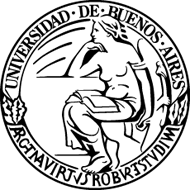
\includegraphics[width=55px,height=50px]{../img/logouba.png}
\hspace{50.7px}

\includegraphics[width=70px,height=50px]{../img/logoCONICET.jpg} 
\hspace{15px}

\includegraphics[width=100px,height=50px]{../img/logoLFP.jpeg}
\end{frame}

















% We want to tag a protein by fusion of a fluorescent protein.
% We known that GFP can provide this (fluorescence) 
% So we decide to use it and we first think a possible construction, made of our target protein(in this case, tubulin), linked to GFP.
% it has been studied that GFP is a relatively small and inert molecule, that doesn't seem to interfere with any biological processes of interest, 
% but the addition of it to can affect the localization or function of the tagged protein
% to prevent this, it is important to use the correct linker sequence, so the whole construction will have the desired properties
% ....OPCIONAL .......  otras coas importantes.....we need to decide if the GFP is added in C or N terminal, that is , the order of the elements....also
\begin{frame}[plain]{Chimeric Proteins}
\begin{adjustwidth}{-2.0em}{-2.0em}
Use of GFP as fluorescent tag\\
\Put(60,-300){ 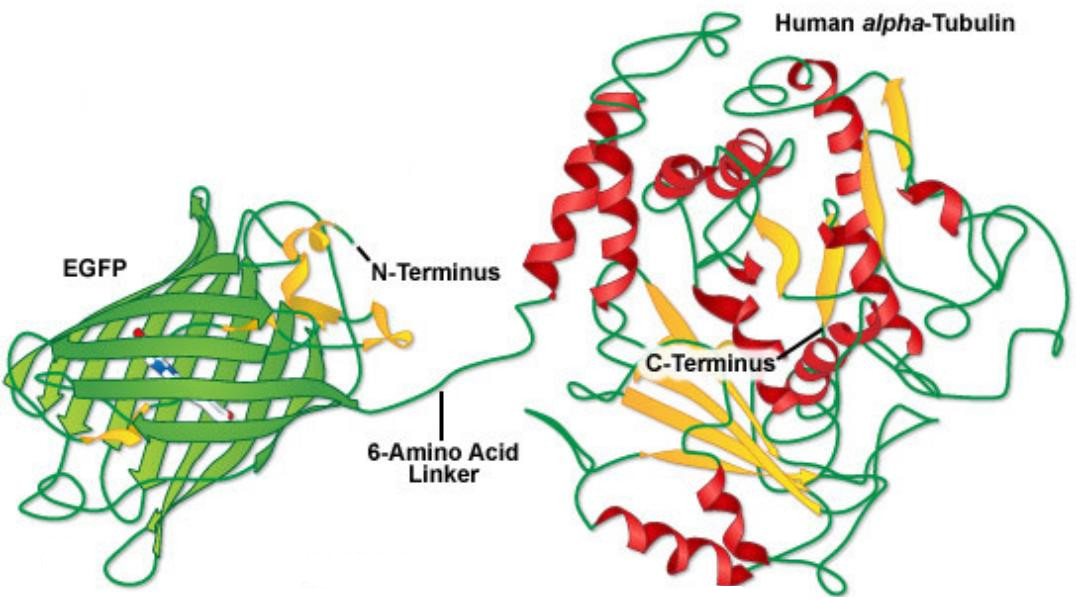
\includegraphics[width=260px]{../img/proteinFusion-GFP-tubulinTransparent.png}}
\\
Construction: GFP + Linker + Tubulin\\
\vspace{145px}
Addition of GFP can affect the localization or function of the tagged protein $\rightarrow$ \textbf{importance of correct linker}
\end{adjustwidth}
\end{frame}










% VIENE DE ......to prevent this, it is important to use the correct linker sequence


% So, a linker is a sequence with a very important function, it (allows the domains to remain)/(it keeps the domains) covalently linked while folding in an independent manner, moving and interacting freely.
% To choose the correct sequence we need to take several aspects(properties) into account: 
% First: length, the sequence needs to allow sufficient distance between units
% Second: the sequence needs to adopt a flexible conformation. This propoerty will allow the units to move and interact freely. To provide this flexibility, the sequence . 
% What is more, this property needs to remain constant, so 

% It is also very important that the linker sequence remains biologically inert. That means we dont want any kind of interaction with molecules that could interfere with normal processes of biological system.

% Finally, the linkers will be part of an experimental process, so there can be some other preferences regarding composition, specifically AAs frequencies, UV silent, net charge.

\begin{frame}{Relevant linker properties}
\vspace{-20px}
\begin{adjustwidth}{-0.5em}{-1.5em}
\textbf{Allows domains to fold independently, move and interact freely}
 \end{adjustwidth}

 \vspace{10px}

\begin{itemize}
  \item Length
  \item Remain in a flexible conformation  %incluye prevencion de aggregation
    \begin{itemize}
     \item Disordered structure, Non-aggregating
    \end{itemize}

  \item Biologically inert  %lack of functional features
    \begin{itemize}
     \item Does not interact with other molecules
    \end{itemize}

  \item Other desirable aspects  %experimental aspects
    \begin{itemize}
     \item AAs frequencies, UV silent, net charge
    \end{itemize}
\end{itemize}
\end{frame}









% At the moment we have 3 different approaches to linker design
% First we can, of course, use linkers extracted from natural multidomain proteins
% We can also propose novel designs containing small and disorder-favoring(disorder-promoting) amino acids.
% Another option is to use different servers available. These servers collect natural and aritificial linkers and provide a search over these set using specific parameters, so the user can find a sequence with the required properties
% (length,    ....)

% We will be able to get different designs but...    , 
% most of the sequences we will get wont have all the desired properties. 
% for example, natural linkers can, of course, have biological functions
% others can have rigid structure
% even if we get sequences with all desired properties, the set of possible designs will be very small, and we will only get a few possible different designs.



\begin{frame}{Current approaches to linker design}
\begin{itemize}

\item Use linkers from natural multi-domain proteins


\item Intuitive design.
 \begin{itemize}
  \item Usually (G/S/P)-rich 
  \end{itemize}
\item Pseudo-Rational design. 
\begin{itemize}
 \item Servers: LINKER, Linkerdb, SynLinker.
\end{itemize}
\end{itemize}
\vspace{20px}
\LARGE{Structure? Inert? Diversity?}
\end{frame}













% Clearly, we dont have a method to design linkers with the correct properties
% but if we have a sequence, we can check any undesired feature by means of different bioinformatic tools available, that can analyze the sequence
% That is, We can predict all unwanted properties.
% OPTIONAL ...That is, we can evaluate (get an idea, get an estimation of) how good or how bad(quality) is a sequence to work as a linker.

% ACA NO DIGO NADA DEL NOMBRE DEL METODO, TOTAL ESTA EN LA DIAPO
% The main idea behind our method is to define a set of tools to check each of the undesired features.
% This evaluation set is composed of: 
% IUPred, to evalute if the sequence will adopt a globular structure
% we have 3 different methods to evaluate sequence propensity to form insluble aggregates
% functional features are evaluated by means of: BLAST(to try to infer function through sequence similarity), also  ELM resource(to find instances of linear motifs), PROSITE(to find functional sites), and ANCHOR(to find recognition elements)
% Finally, some optional evaluations are:
%      check the presence of ultraviolet aboserbers aminoacids W(Tryptophan), Y(Tyrosine), F(Phenylalanine)
% 	and check the presence of charged residues.


% so....what do we do with this evaluation set?

% 
% DECIR QUE TODOS LOS MÉTODOS DAN INFORMACION A NIVEL DE POSICION DENTRO DE LA SECUENCIA
%  any of these methods allows to define if a particular position contains a specific negative aspect 
% each of these methods allows to asses if a particular position has that specific negative aspect we are evaluating
% so we can define a scoring function

\begin{frame}{Rational approach}
 
PATENA uses different applications to evaluate a candidate linker.
\vspace{15px}

\begin{tabular}{l|l}
\textbf{Undesired feature} & \textbf{Prediction method} \\ \hline \hline
\rowcolor{Gray} Globular structure & IUPred  \\
Insoluble aggregates & TANGO, PASTA, WALTZ   \\
\rowcolor{Gray}Functional features & BLAST, ELM, PROSITE, ANCHOR \\  
UV absorption(OPTIONAL) & W, Y, F \\ %Presence of UV-absorbers residues \\
\rowcolor{Gray}Net charge(OPTIONAL)& Presence of charged residues\\
\end{tabular}
 

\vspace{20px} 
Each of these methods allows to predict the presence of undesired features at specific position $\rightarrow$ define a scoring function
\end{frame}








% this is an example of application of this scoring function
% each tool provides a value of 1 for each position that has undesired feature. 
% summing up all the values for each position we have a position score, defining the total number of undesired features for it
% and finally, if we add all the position scores we can get a global score.
% so we have a function, defining a value of how bad is a linker. what can we do with it? ..... ****SWITCH

% *********************************************
%      EJEMPLO DE EVALUACION DE SCORE
% *********************************************
% 
\begin{frame}{Scoring example}
 \begin{tabular}{llllllllllllll} 
\hline
\rowcolor{GrayOscuro}Sequence & \textbf{M} & \textbf{V} & \textbf{L} & \textbf{S} & \textbf{P} & \textbf{A} & \textbf{D} & \textbf{K} & \textbf{T} & \textbf{N} & \textbf{P} & \textbf{D} \\ \hline \hline
 
% Puntaje Inicial & 0 & 0 & 0 & 0 & 0 & 0 & 0 & 0 & 0 & 0 & 0 & 0\\ \hline
\rowcolor{Gray}IUPred           	& 0 & 1 & 1 & 1 & 1 & 0 & 0 & 1 & 1 & 1 & 0 & 0\\ \hline  
TANGO 		       			& 1 & 1 & 1 & 1 & 0 & 0 & 0 & 0 & 0 & 0 & 0 & 0\\ \hline  
\rowcolor{Gray}PASTA			& 1 & 1 & 0 & 0 & 0 & 0 & 0 & 1 & 0 & 1 & 1 & 1\\ \hline  
ELM          	      			& 0 & 1 & 1 & 0 & 0 & 0 & 0 & 1 & 1 & 1 & 1 & 1\\ \hline 
\rowcolor{Gray}BLAST			& 1 & 0 & 1 & 1 & 1 & 0 & 0 & 0 & 0 & 1 & 1 & 1\\ \hline 
PROSITE 	      			& 0 & 0 & 1 & 0 & 0 & 0 & 0 & 0 & 0 & 1 & 1 & 1\\ \hline 
\rowcolor{Gray}ANCHOR	        	& 1 & 1 & 1 & 0 & 0 & 0 & 0 & 0 & 0 & 1 & 0 & 1\\ \hline \hline
\rowcolor{GrayOscuro}Position score     & 4 & 5 & 6 & 3 & 2 & 0 & 4 & 3 & 2 & 6 & 4 & 5\\ \hline
\rowcolor{GrayOscuro}Global Score  & 44 &&&&&&&&&&& \\ \hline
\end{tabular}
\end{frame}








% So, we have seen the core of PATENA, which is the use of a scoring function to evaluate undesired features of linker sequences
% We now will see how PATENA use this function to implement a linker design method.

% to use this method the user will need to provide a candidate linker , or just the length. 

% as a result, the user will get a sequence which has no undesired features. that is, a sequence with score equal to zero.
% this resulting design can be used as linker

% As you can see, if the user only defines the length of the sequence, this method can design a linker from scratch. 

% lets see more in detail how this method works, using the scoring function to implement an optimization method

\begin{frame}{PATENA: Input - Output}

% \centering
\vspace{24px}
\begin{adjustwidth}{-2.0em}{-2.0em}
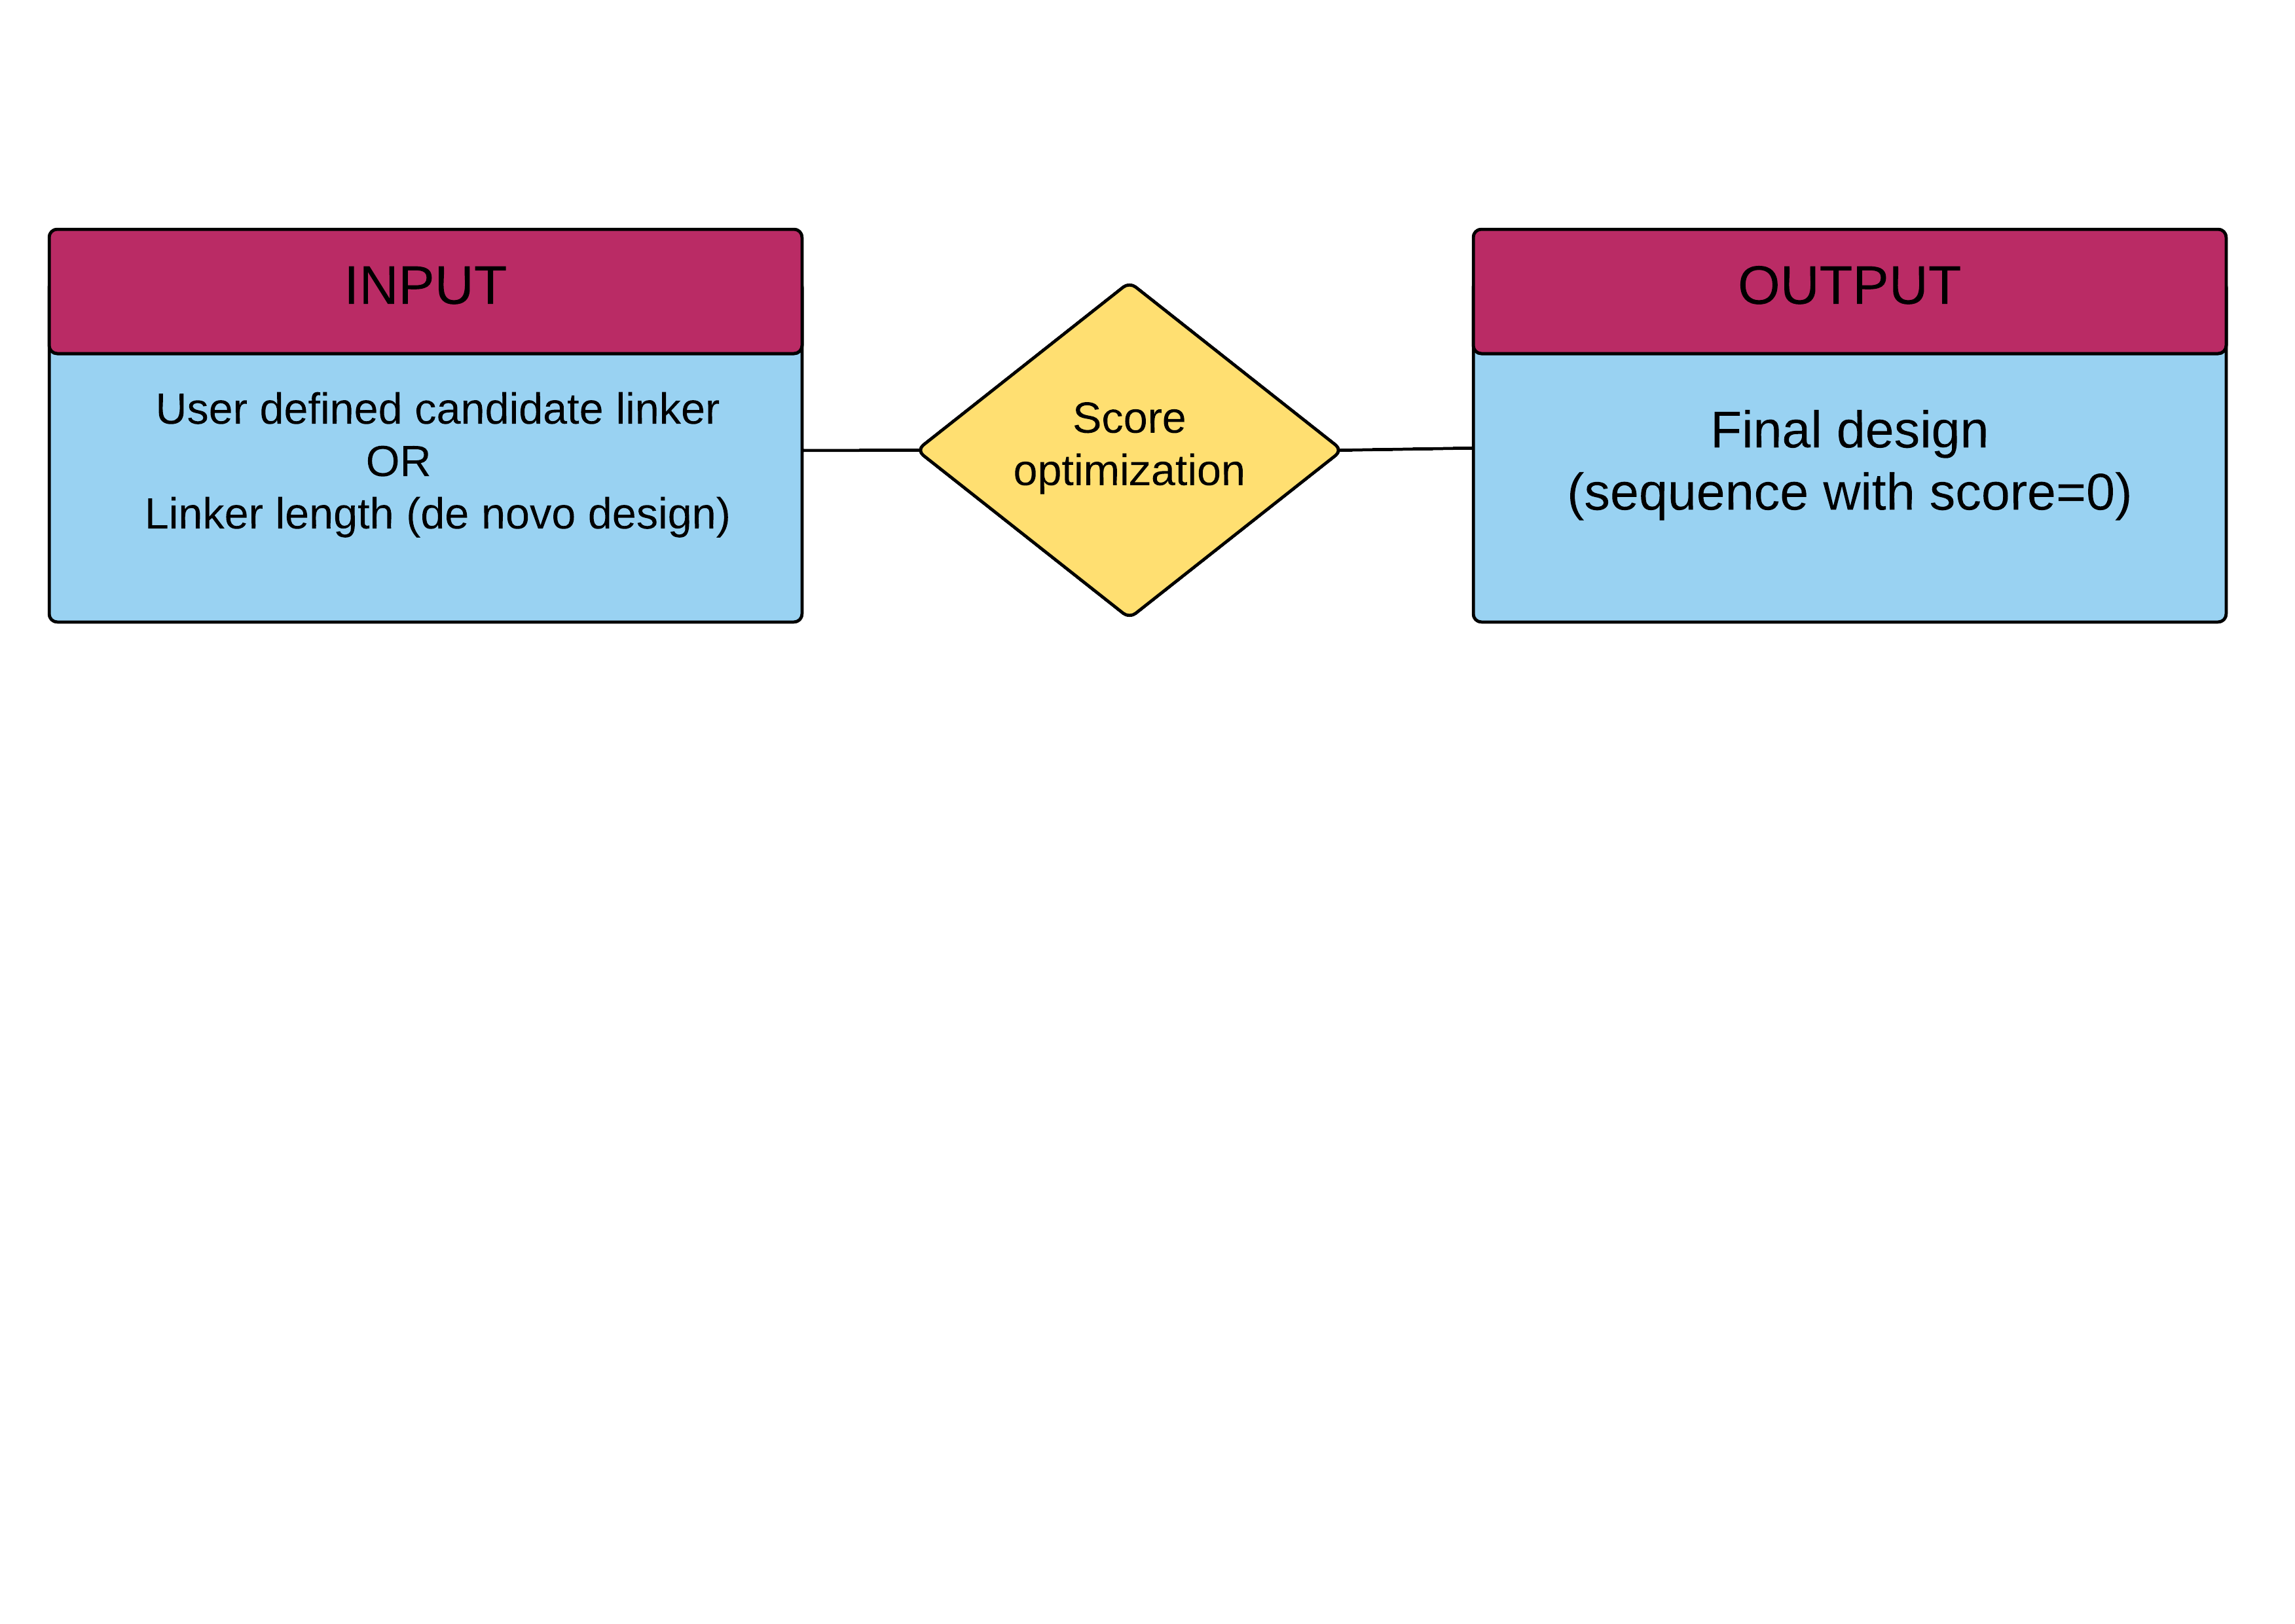
\includegraphics[width=350px]{../img/patenaCoarseGrained.png}
 
\end{adjustwidth}


\end{frame}







% The method starts defining an initial sequence, this sequence can be a users input, or if the user defined a length, a random sequence is created.
% Once we have a starting sequence, we make a first score evaluation.
% If the score is greater than zero, we have some undesired features, in this case we propose a point mutation, aiming at the high scoring positions, that is, the positions that accumulate most undesired features.
% We evaluate this proposition, again using the scoring function.
% If this mutation decreases the score, then we will incorporate that into the sequence.
% The heuristic decision is implemented using a method known as Monte Carlo decision. This decision is based on the score difference and on a beta parameter, which is proportional to the acceptance rate.
% Based on this decision we can accept the mutation or not.

% What we have here is, again, an optimization of the scoring function.
% Once we have this algorithm implemented we need to see if we can find an effective beta value that will allow the execution to efficiently find a design.


% *********************************************
%      ESQUEMA GRAFICO DE PATENA
% *********************************************
\begin{frame}[plain]{PATENA method}
% \vspace{-0.5\baselineskip}
\begin{adjustwidth}{-2.0em}{-2.0em}
% \begin{adjustheight}{-1.5em}{-1.5em}
% 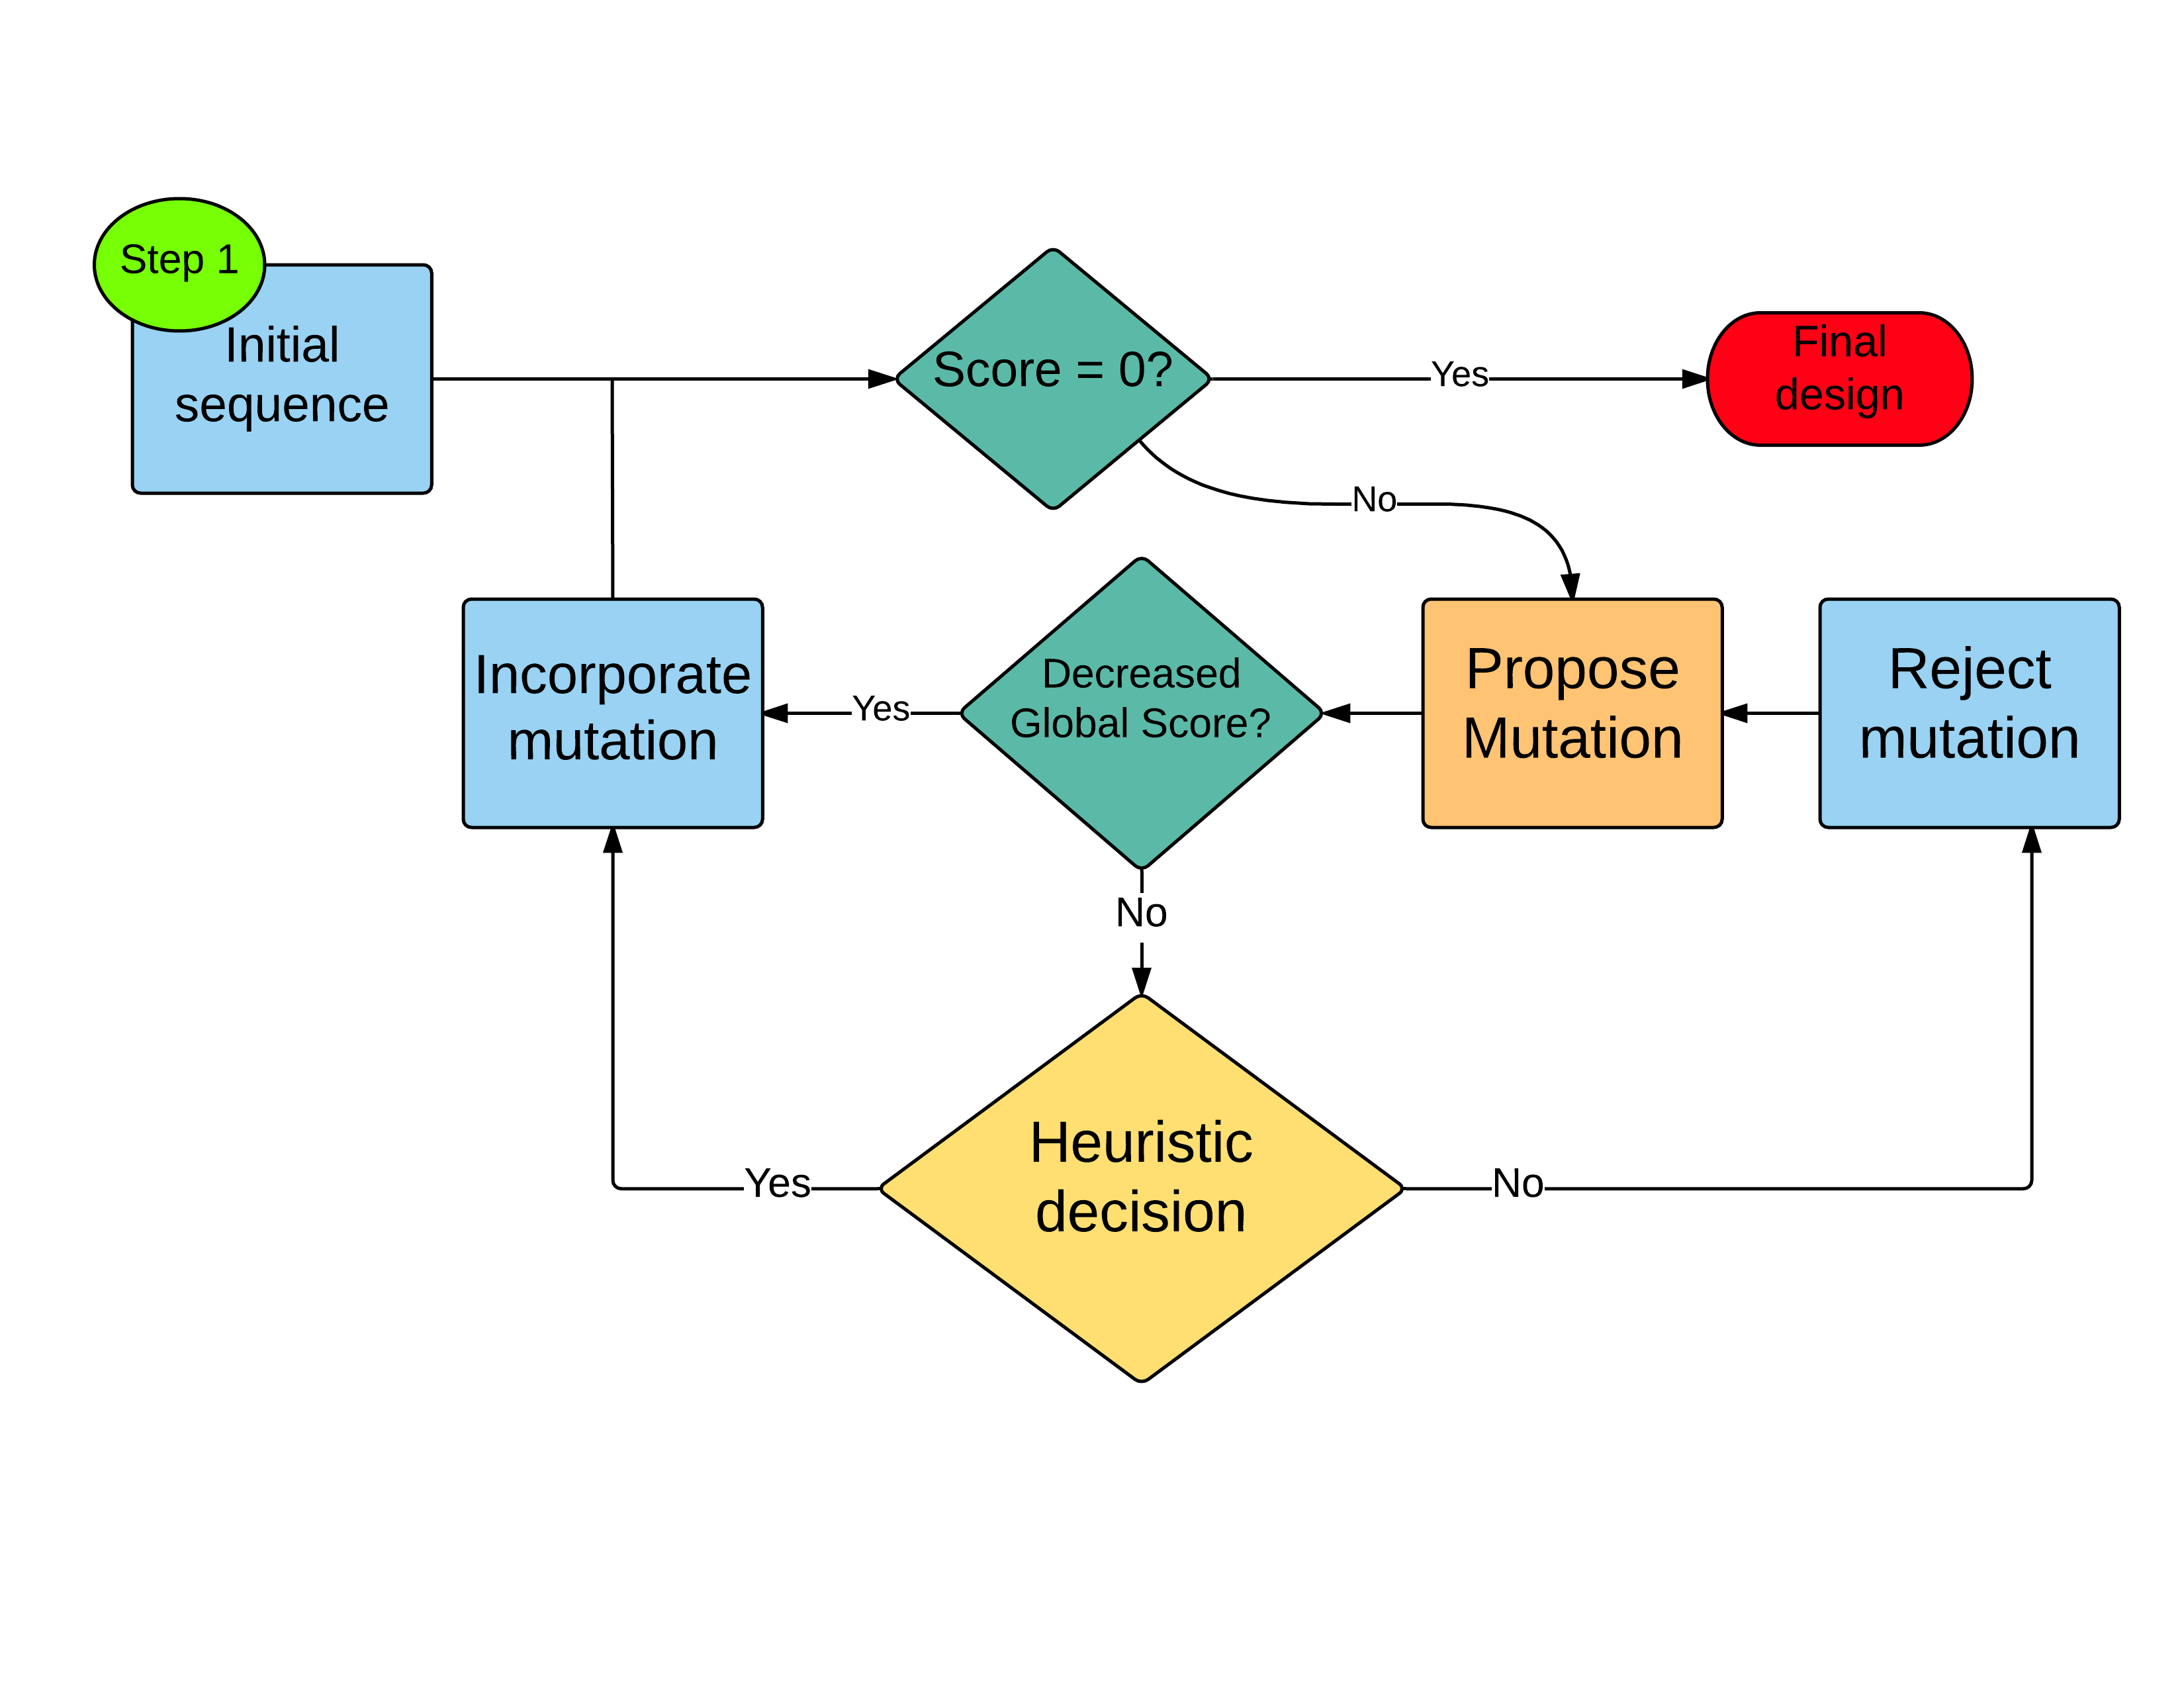
\includegraphics[width=350px,height=250px]{../img/patenaReduced.png} 
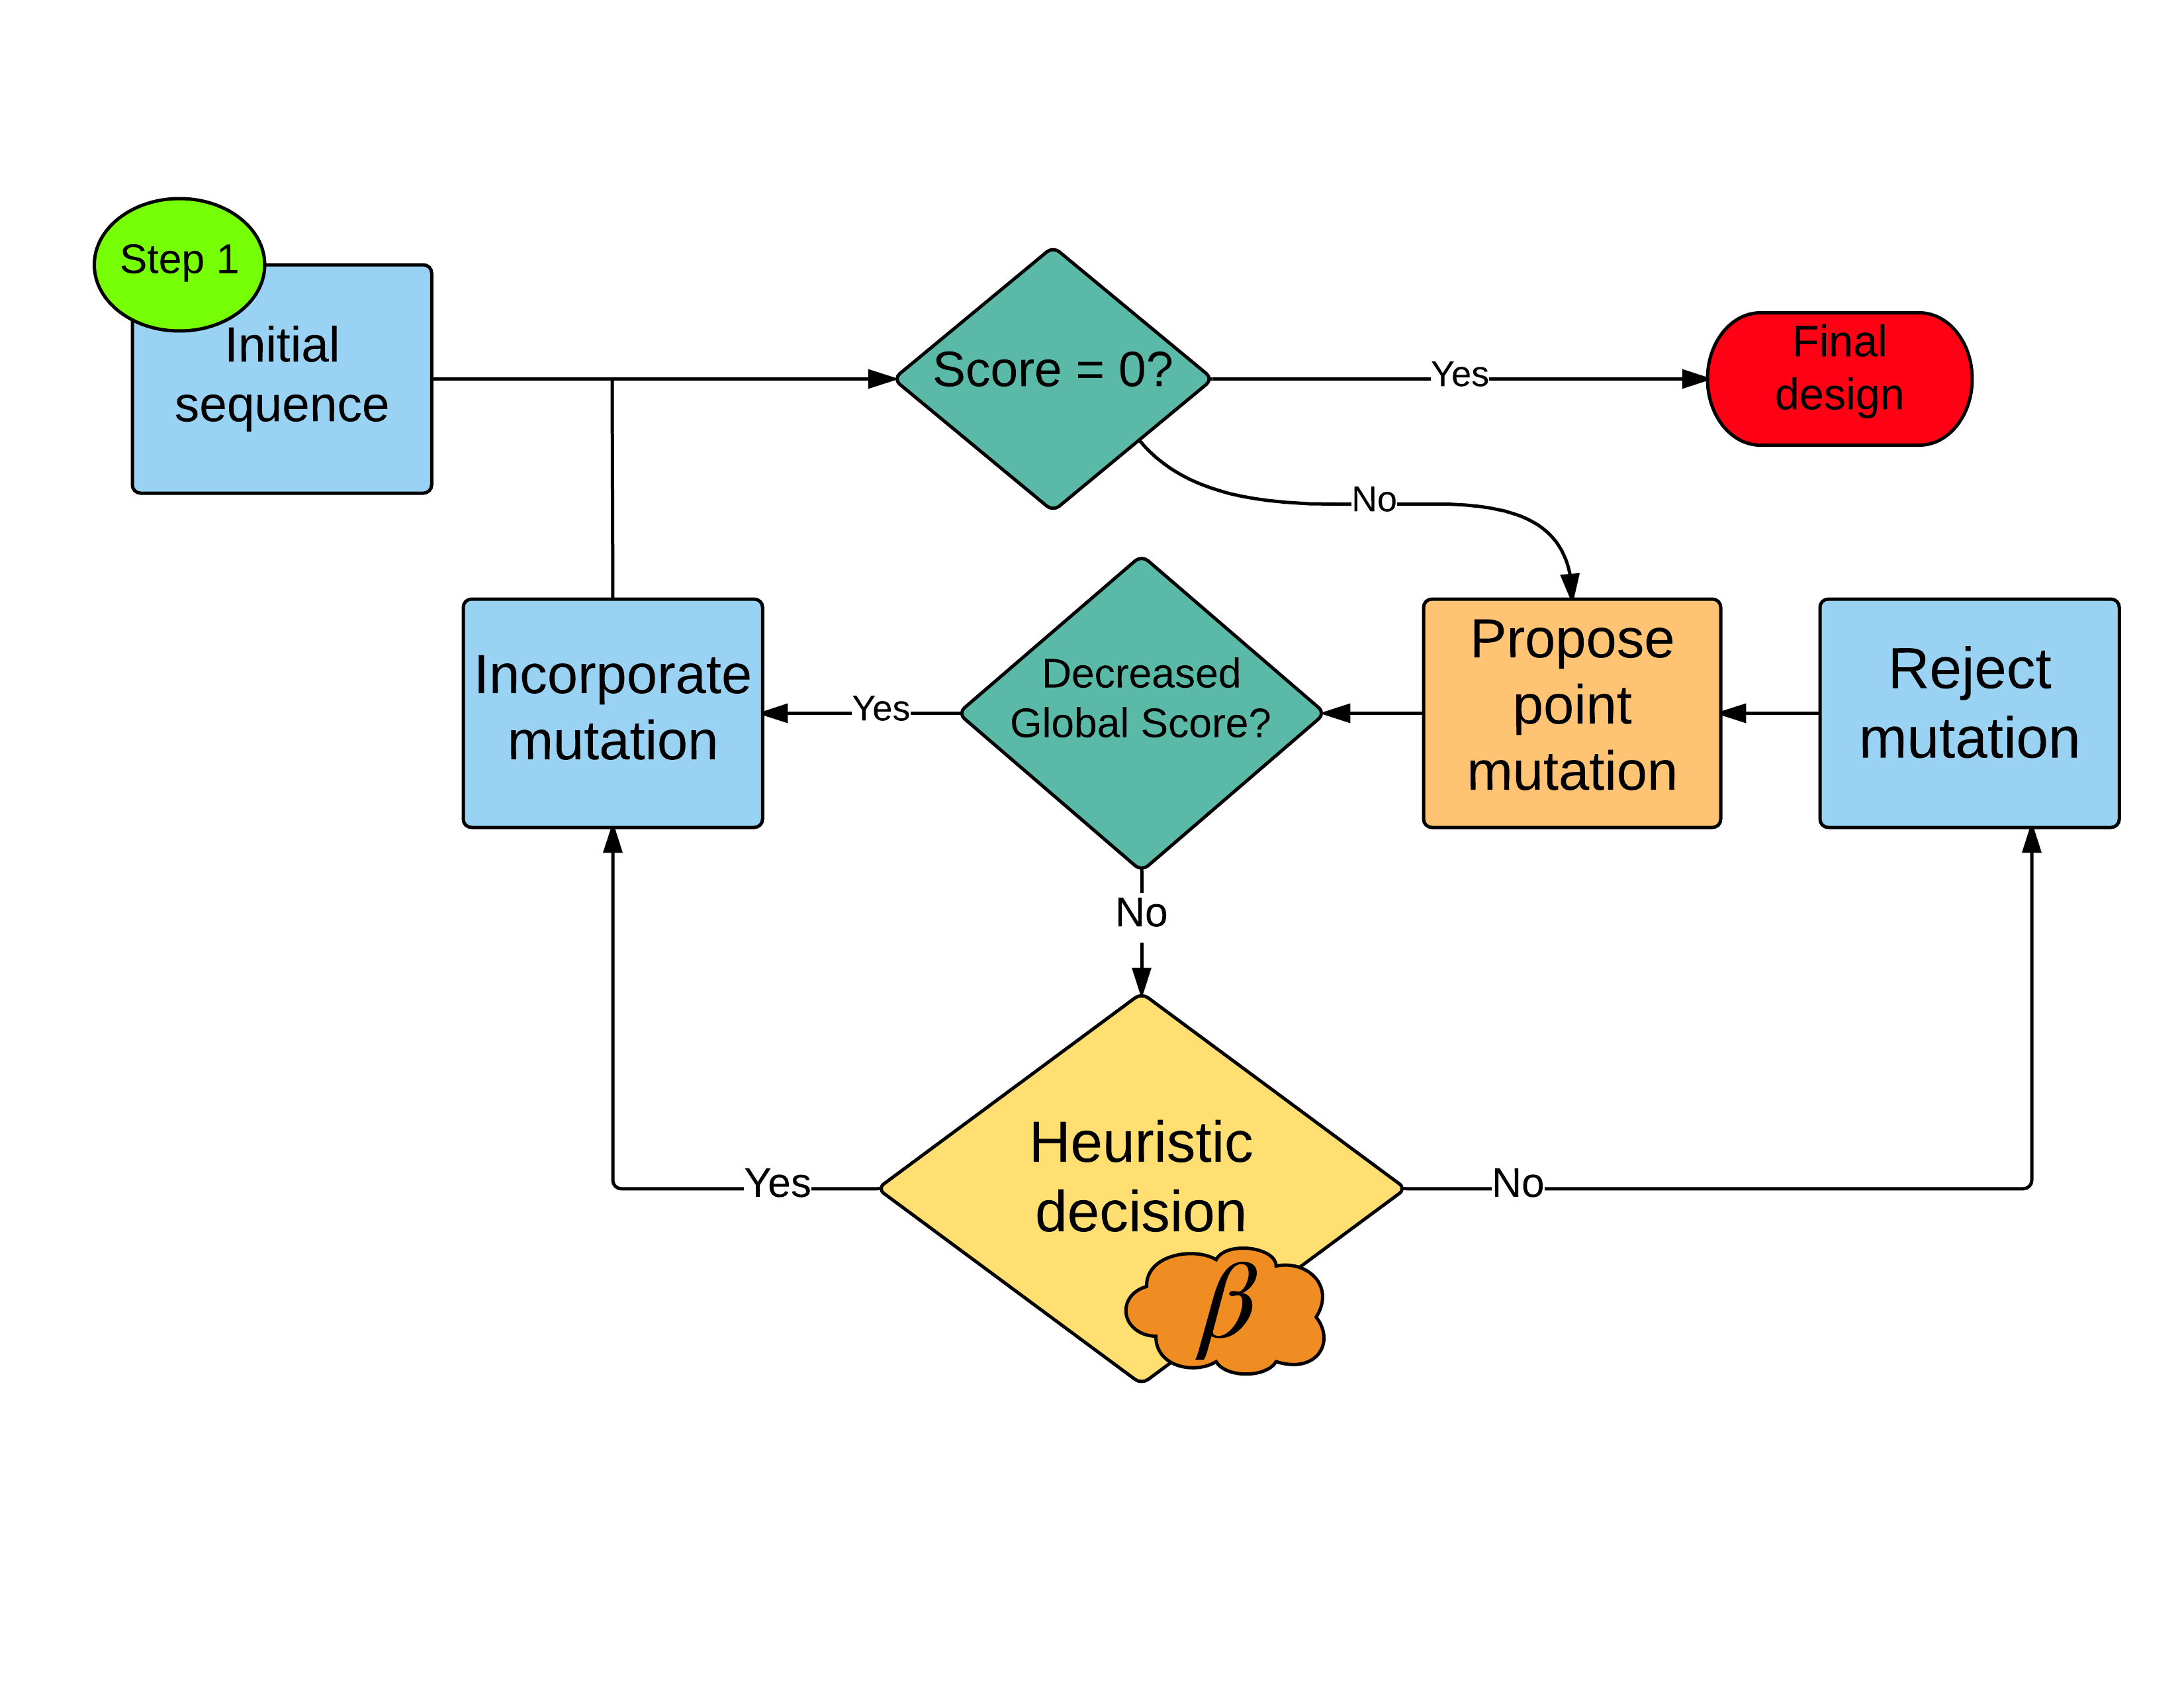
\includegraphics[width=350px,height=250px]{../img/patenaReduced-Beta.png} 
% \end{adjustheight}
\end{adjustwidth}
% \vspace{-\baselineskip}
\end{frame}























% 
%

% The execution can find designs in all cases but we see that the effective range is located below  beta value of 2.0
% Just to move on with evaluation we choose a beta of 1.0, which is in the middle. This is just a decision we made.

% *********************************************
%      BETA vs TIME
% *********************************************
\begin{frame}[plain]{Effective $\beta$ range $\approx$ [0.1 - 2.0]}
\centering
% Optimal $\beta$ range  
[Length = 50] - [Random (n=3) and Natural (n=3) seq. / each $\beta$] \\
\begin{adjustwidth}{-1.5em}{-2.5em}
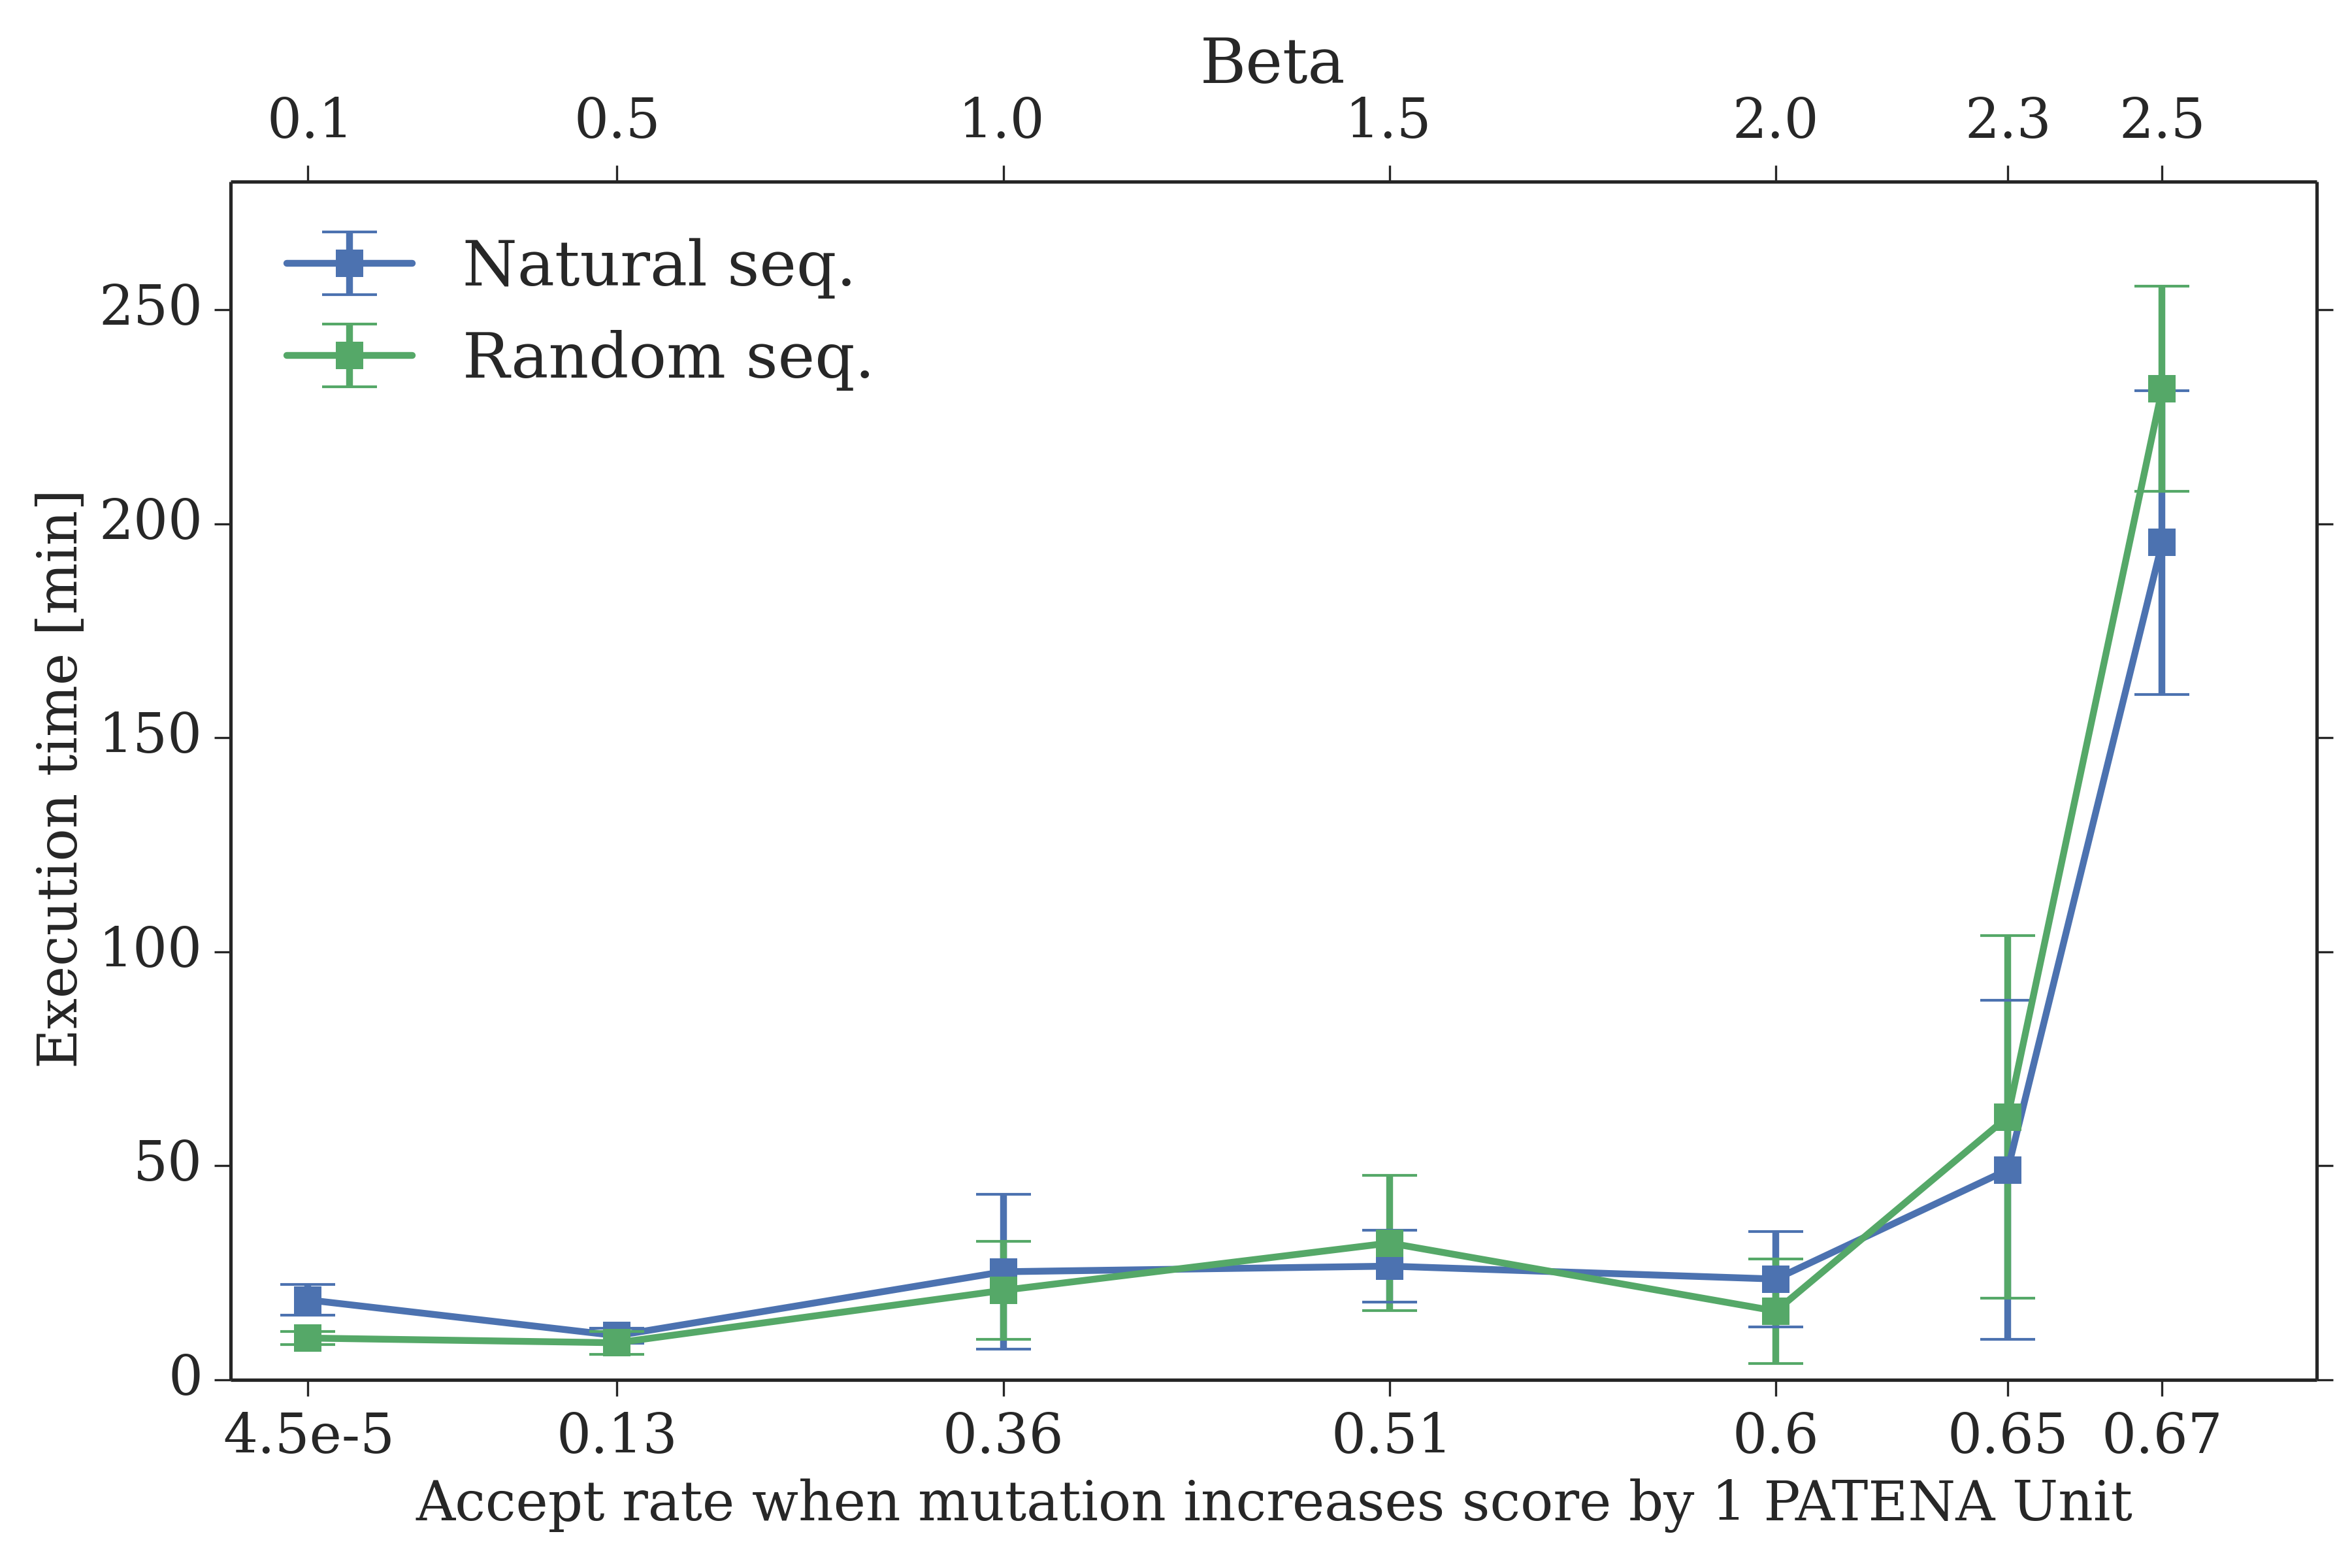
\includegraphics[width=330px,height=210px]{../img/beta-vs-time-length50-300dpi.png} 
\end{adjustwidth}
\end{frame}
















% we know it works and we have one effective value for beta.
% In this case, the execution profile is something like this.
% this graphic is only to get a better idea of how the execution profile looks like.
% how many mutations are required? in this particular execution we have a bit more than two hundred mutations 
% This number will be variable, since the method has some heuristics behind so it is not deterministic and it of course depends in the initial sequence and the length if it...
% that is an important aspect, what happens if we variate the length of the sequence??.....ACA ENGANCHO CON EL PROX. SLIDE
% 
% ***************************************************************
%      SCORE vs MUTACION  PARA 1 SOLA EJECUCION USANDO BETA=1.0
% ****************************************************************
\begin{frame}[plain]{Sample execution profile using defined $\beta$ (1.0)}
% \vspace{-0.5\baselineskip}
\begin{adjustwidth}{-1.5em}{-2.5em}
\centering

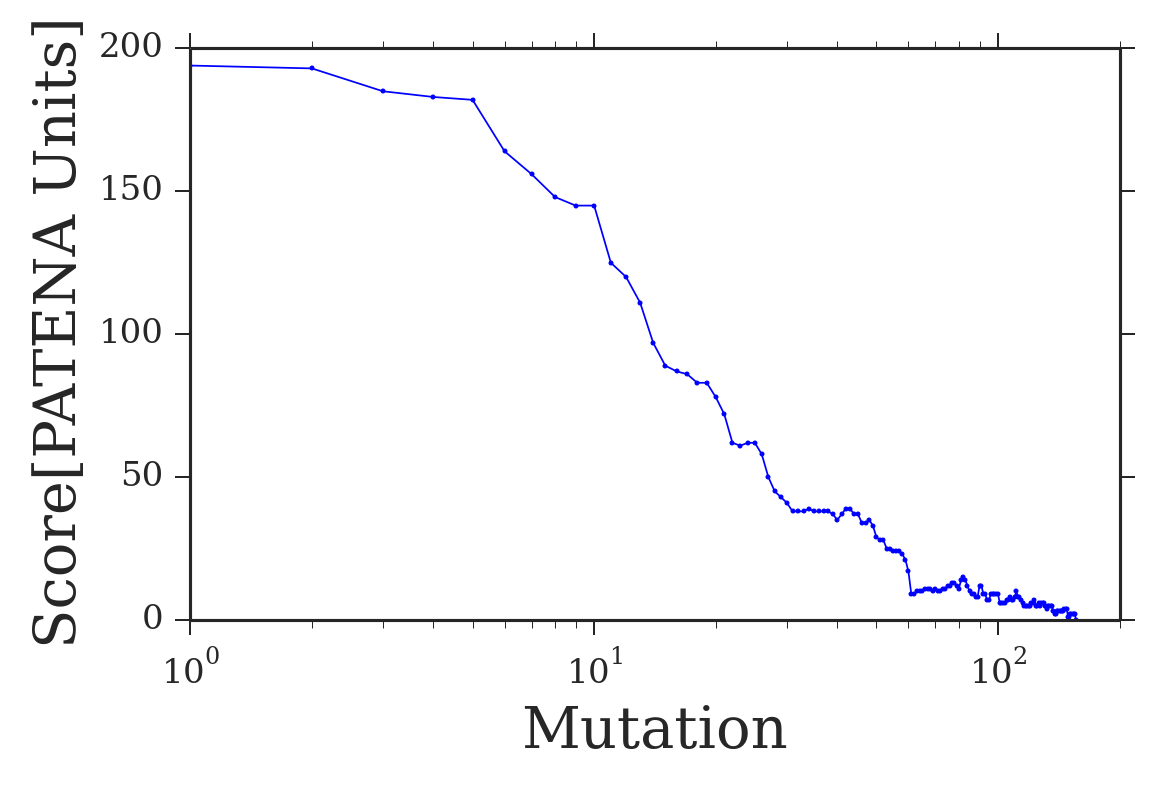
\includegraphics[width=330px,height=210px]{../img/iterationVsScore-individualBeta1-EXAMPLE.png}
% 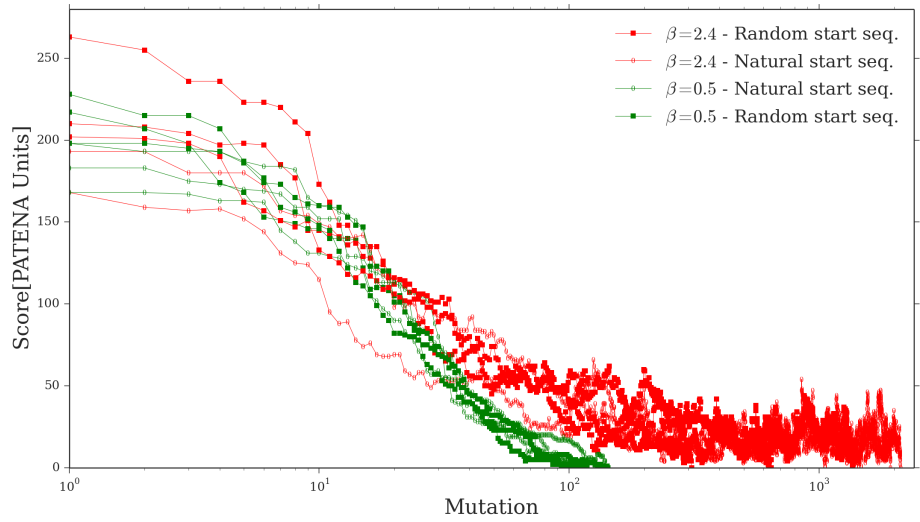
\includegraphics[width=330px,height=210px]{../img/scoreVsMutation-individual.png} 

\end{adjustwidth}
% \vspace{-\baselineskip}
\end{frame}








% to evaluate this we made a total of 36 different executions, starting from natural and random sequences of diffferent lengths.
% 

% *********************************************
%      TIEMPO EJECUCION vs LENGTH SECUENCIA
% *********************************************
\begin{frame}[plain]{Approximate linear dependence with length}
\centering
% Optimal $\beta$ range  
% [Length = 30] - [Random (n=3) and Natural (n=3) seq. / each $\beta$] \\
\begin{adjustwidth}{-1.5em}{-2.5em}
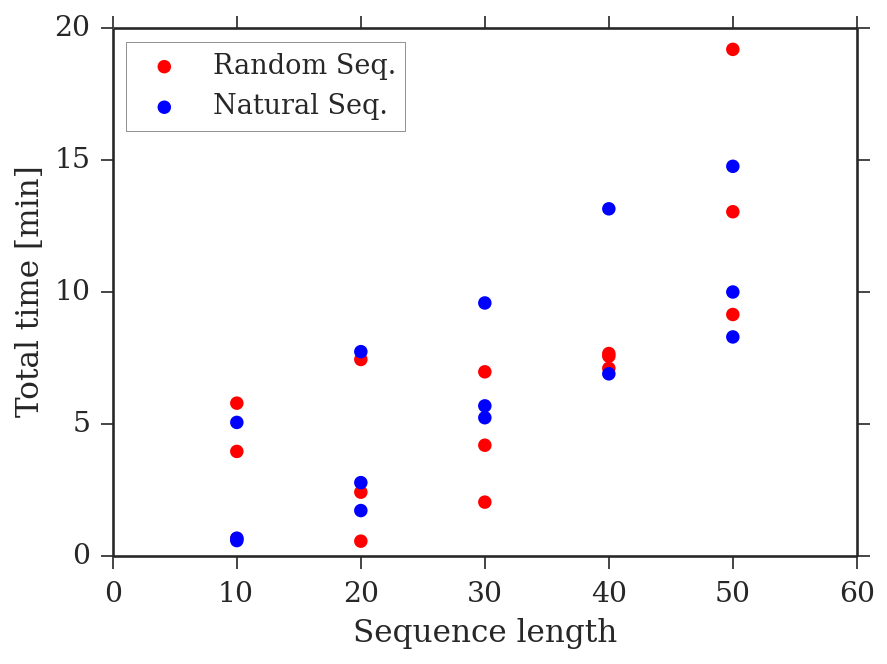
\includegraphics[width=330px,height=210px]{../img/lengthVsTime.png} 
\end{adjustwidth}
\end{frame}







% *********************************************
%      DIVERGENCIA: dividido en 2 slides
% *********************************************% 
% 
% 	DECIR SIEMPRE IDENTITY , PORQUE SI DIGO SIMILARITY SE CONFUNDE CON ALINEAMIENTO , ETC, ETC
% 		ACLARAR QUE COMO LOS RESULTADOS TIENEN LA MISMA LONGITUD, LA IDENTIDAD SE EVALUA SIMPLEMENTE COMPARANDO QUE POSICIONES TIENEN EXACTAMENTE EL MISMO RESIDUO
% 



% So, at the moment we have a method that allows to, at least, get some resulting designs.
% Since it is a Nondeterministic algorithm it could allow to get a diverse set of results.
% (OPTIONAL) but i said first that one of the problems with linker design methods nowadays is that they 
% lets see what kind of results we get, to see how different are the results ?
% Here we have identity between a set of results(a total of 74 designs) obtained from running PATENA using the same initial sequence(these are the green bars).
% We have also blue bars indicating the identity that can be found between random sequences of the same length
% Conclusion: we can see, that, identity between resulting designs is greater than that between random sequences. Nevertheless the set of results is clearly heterogeneous.

% It is great to have such diversity but, if the user defines a sequence to start, the idea is to get a at least some similarity in the resulting design. 
% how similar are these results with the initial sequence??  ******** SWITCH DIAPO
\begin{frame}[plain]{Nondeterministic algorithm: same input $\rightarrow$ different results}
\centering
\vspace{10px}
\begin{adjustwidth}{-2.5em}{-2.5em}
\hspace{10px} 
Fixed starting sequence $\rightarrow$ 74 designs - Identity \textbf{between final sequences}
% mayor que random pero claramente heterogeneas
\end{adjustwidth}
\hspace{10px} 
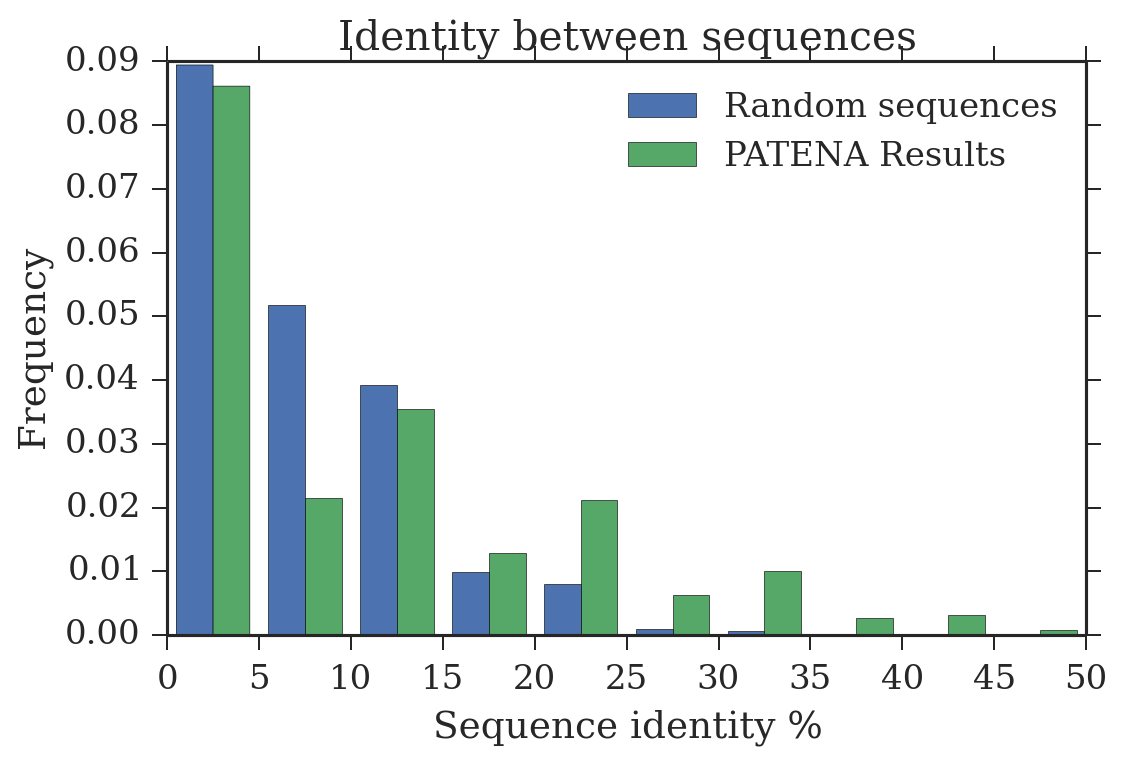
\includegraphics[width=275px,height=215px]{../img/againstAll-random.png}
% 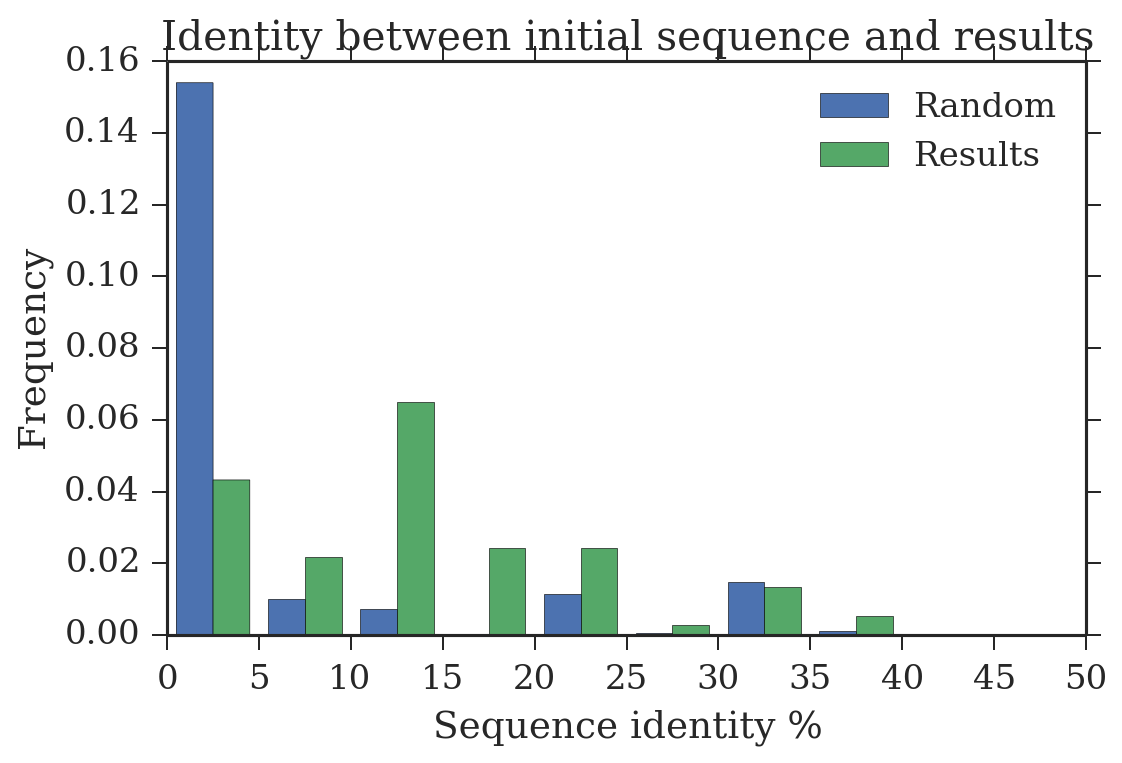
\includegraphics[width=175px,height=145px]{../img/againstInitial-random.png}
\end{frame}



% Using the same set of results we show here(in green bars) the identity between the set of results and the initial sequence.
% blue bars show the identity between that initial sequence and a set of random sequences of the same length
% Conclusion: the resulting set, although is quite diverse, still maintain certain similarity with initial sequence.
\begin{frame}[plain]{Nondeterministic algorithm: same input $\rightarrow$ different results}
\centering
\vspace{10px}
\begin{adjustwidth}{-2.5em}{-2.5em}
\hspace{10px}
Fixed starting sequence $\rightarrow$ 74 designs - Identity \textbf{with initial sequence}
% mayor que random pero claramente hubo bastantes mutaciones
\end{adjustwidth}
\hspace{10px}
% 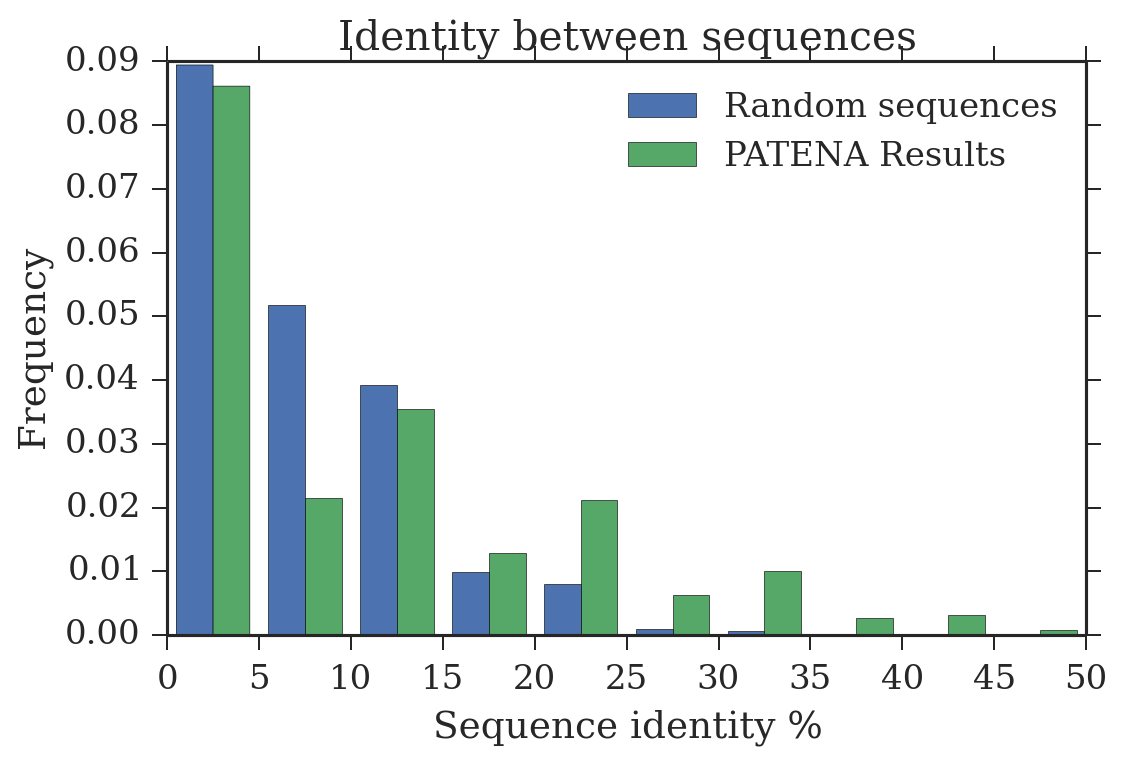
\includegraphics[width=175px,height=145px]{../img/againstAll-random.png}
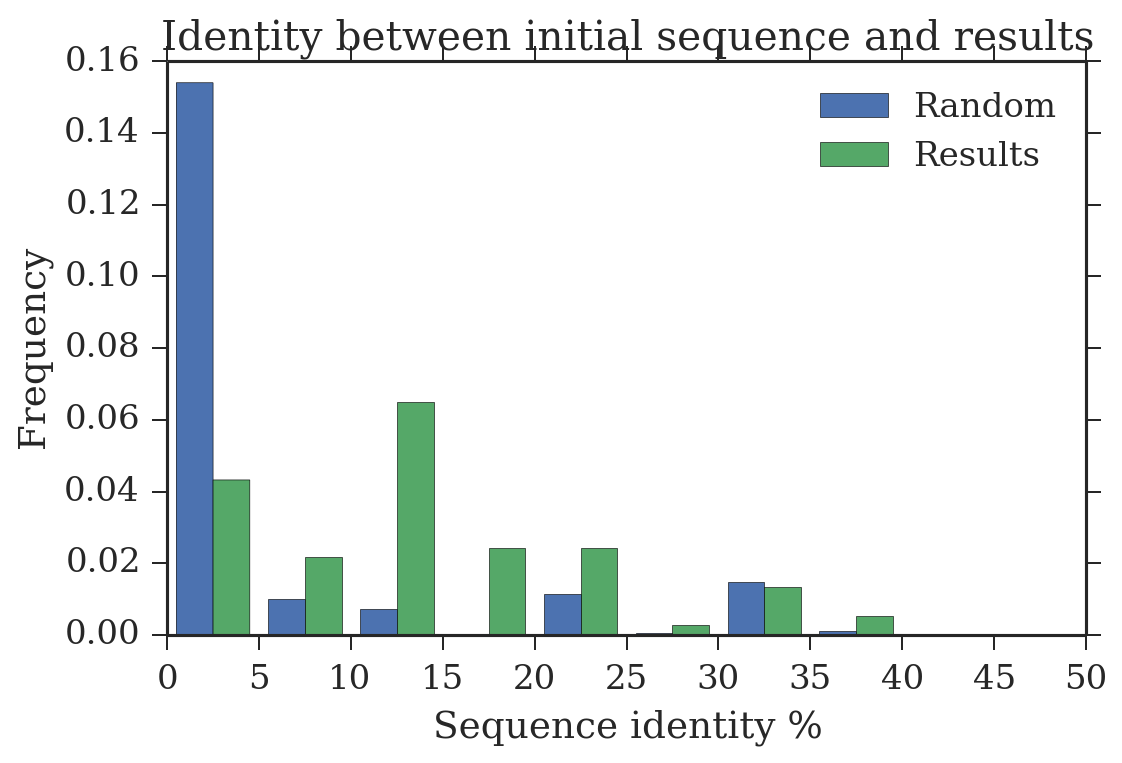
\includegraphics[width=275px,height=215px]{../img/againstInitial-random.png}
\end{frame}







% To sum everything up
% PATENA can find suitable linkers in a short execution time, that is, in the order of tens of minutes usually
% We can also obtain a set of designs showing high diversity, which is ideal since we can fill lot of different preferences.
% The input can be very simple so this method allows to develop a server to easily obtain linker designs. 
\begin{frame}{Conclusion}
\begin{itemize}
 \item PATENA can find suitable protein linkers in a short execution time.
 \item The set of designs that can be obtained from the same sequence shows high diversity. 
 \item Allows for development of server to design linker sequences.
%  \item We interpret that the space of suitable linker sequences is a large fraction of the whole sequence space.
\end{itemize}
\end{frame}


























% *************************************************************
% *************************************************************
% *************************************************************
% 			EXTRA
% *************************************************************
% *************************************************************
% *************************************************************







% *************************************************************
% 		SEQUENCE LOGO  
% *************************************************************

\begin{frame}
\centering
Fixed starting sequence $\rightarrow$ 74 designs\\
\begin{adjustwidth}{-1.5em}{-2.5em}
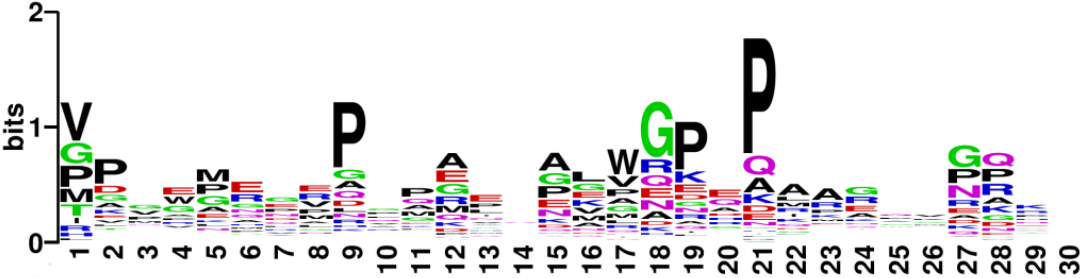
\includegraphics[width=340px,height=150px]{../img/logo.png}\\ 
\vspace{10px}
\hspace{18px}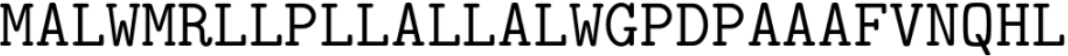
\includegraphics[width=325px,height=15px]{../img/sequence.png}
\end{adjustwidth}
\end{frame}

\begin{frame}
\begin{adjustwidth}{-1.5em}{-2.5em}
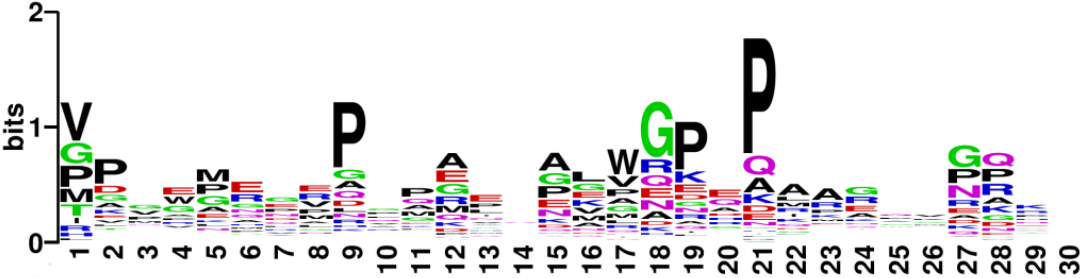
\includegraphics[width=340px,height=150px]{../img/logo.png}\\ 
% \vspace{10px}
\hspace{18px}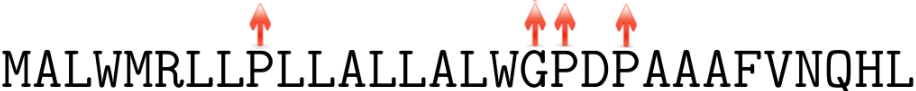
\includegraphics[width=325px,height=25px]{../img/sequence2.png}
\end{adjustwidth}
\end{frame}










% *************************************************************
%      OBSERVED FREQUENCY vs EXPECTED FREQUENCY
% *************************************************************
\begin{frame}
% {Standard composition deviation}
\centering
Standard composition
% Fixed starting sequence $\rightarrow$ 74 designs\\
\begin{adjustwidth}{-1.5em}{-2.5em}
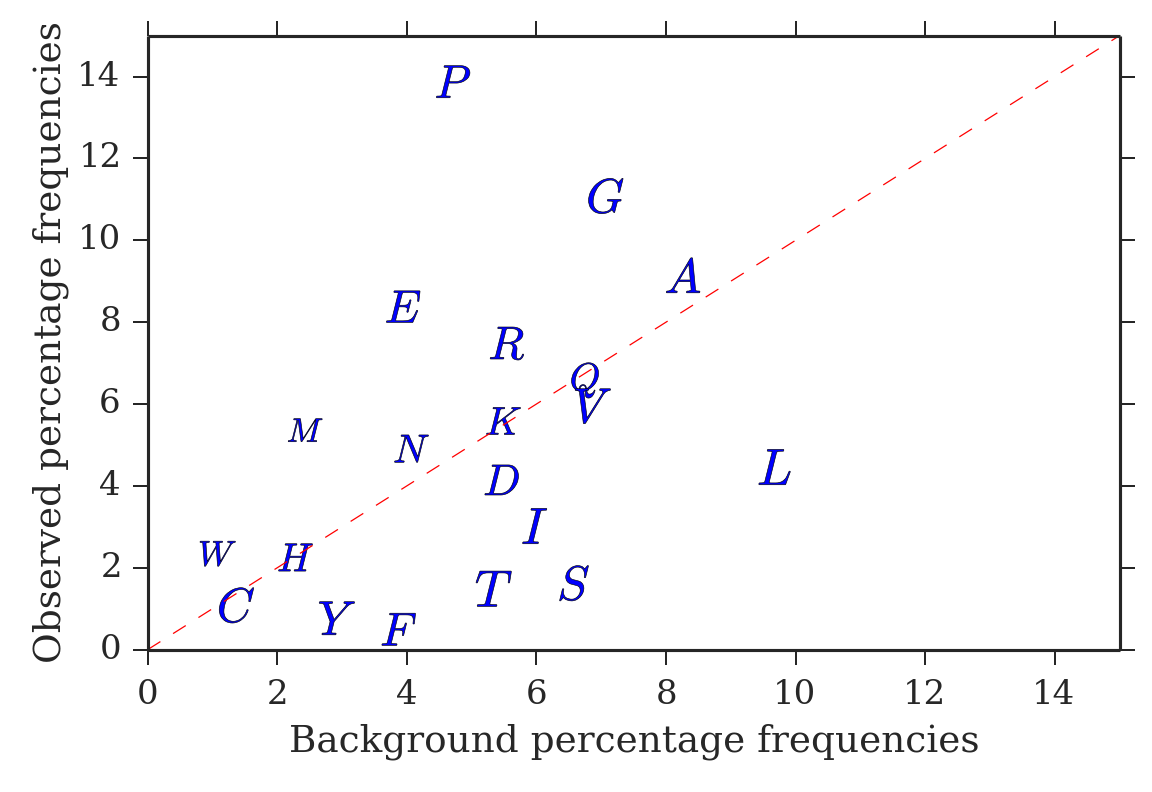
\includegraphics[width=340px,height=250px]{../img/frequenciesComparison.png}\\ 
\end{adjustwidth}
\end{frame}












% *************************************************************
% 		BETA  vs  MUT. ATTEMPTS + ITERATIONS
% *************************************************************
\begin{frame}
\begin{adjustwidth}{-1.5em}{-2.5em}
% 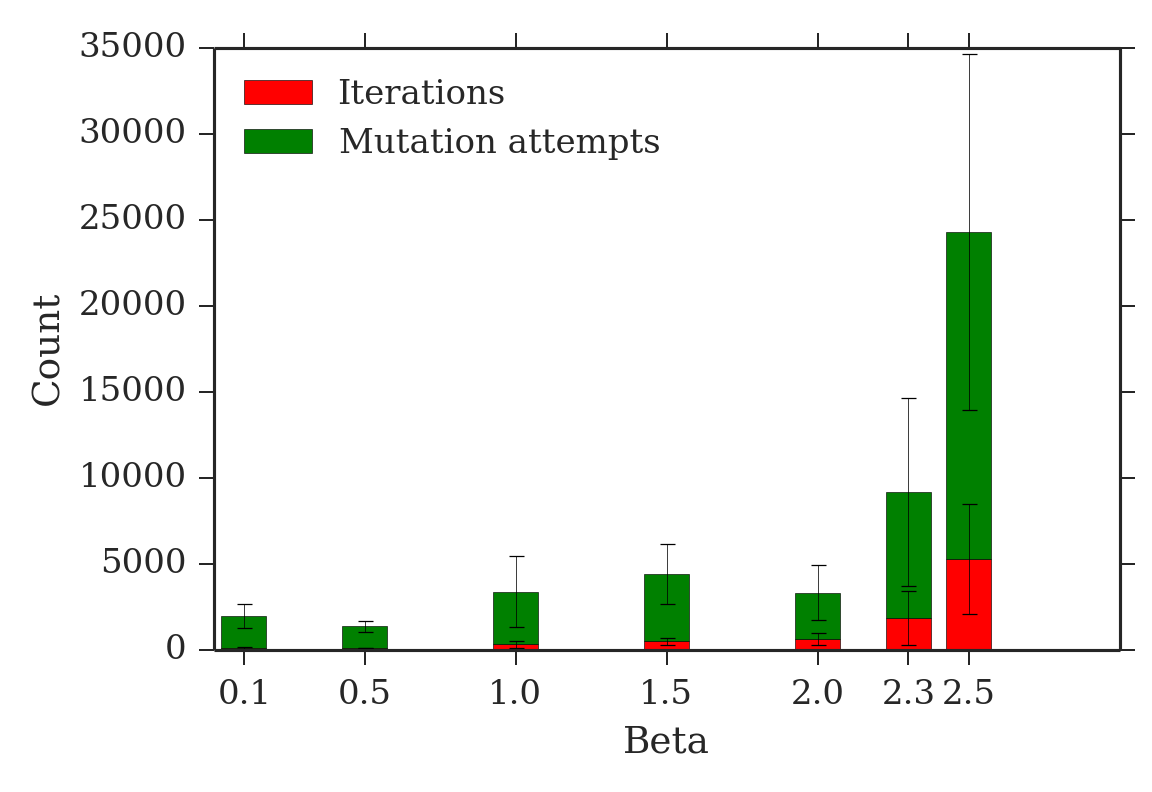
\includegraphics[width=340px,height=250px]{../img/betaVsIterations-MutAttempts.png}\\
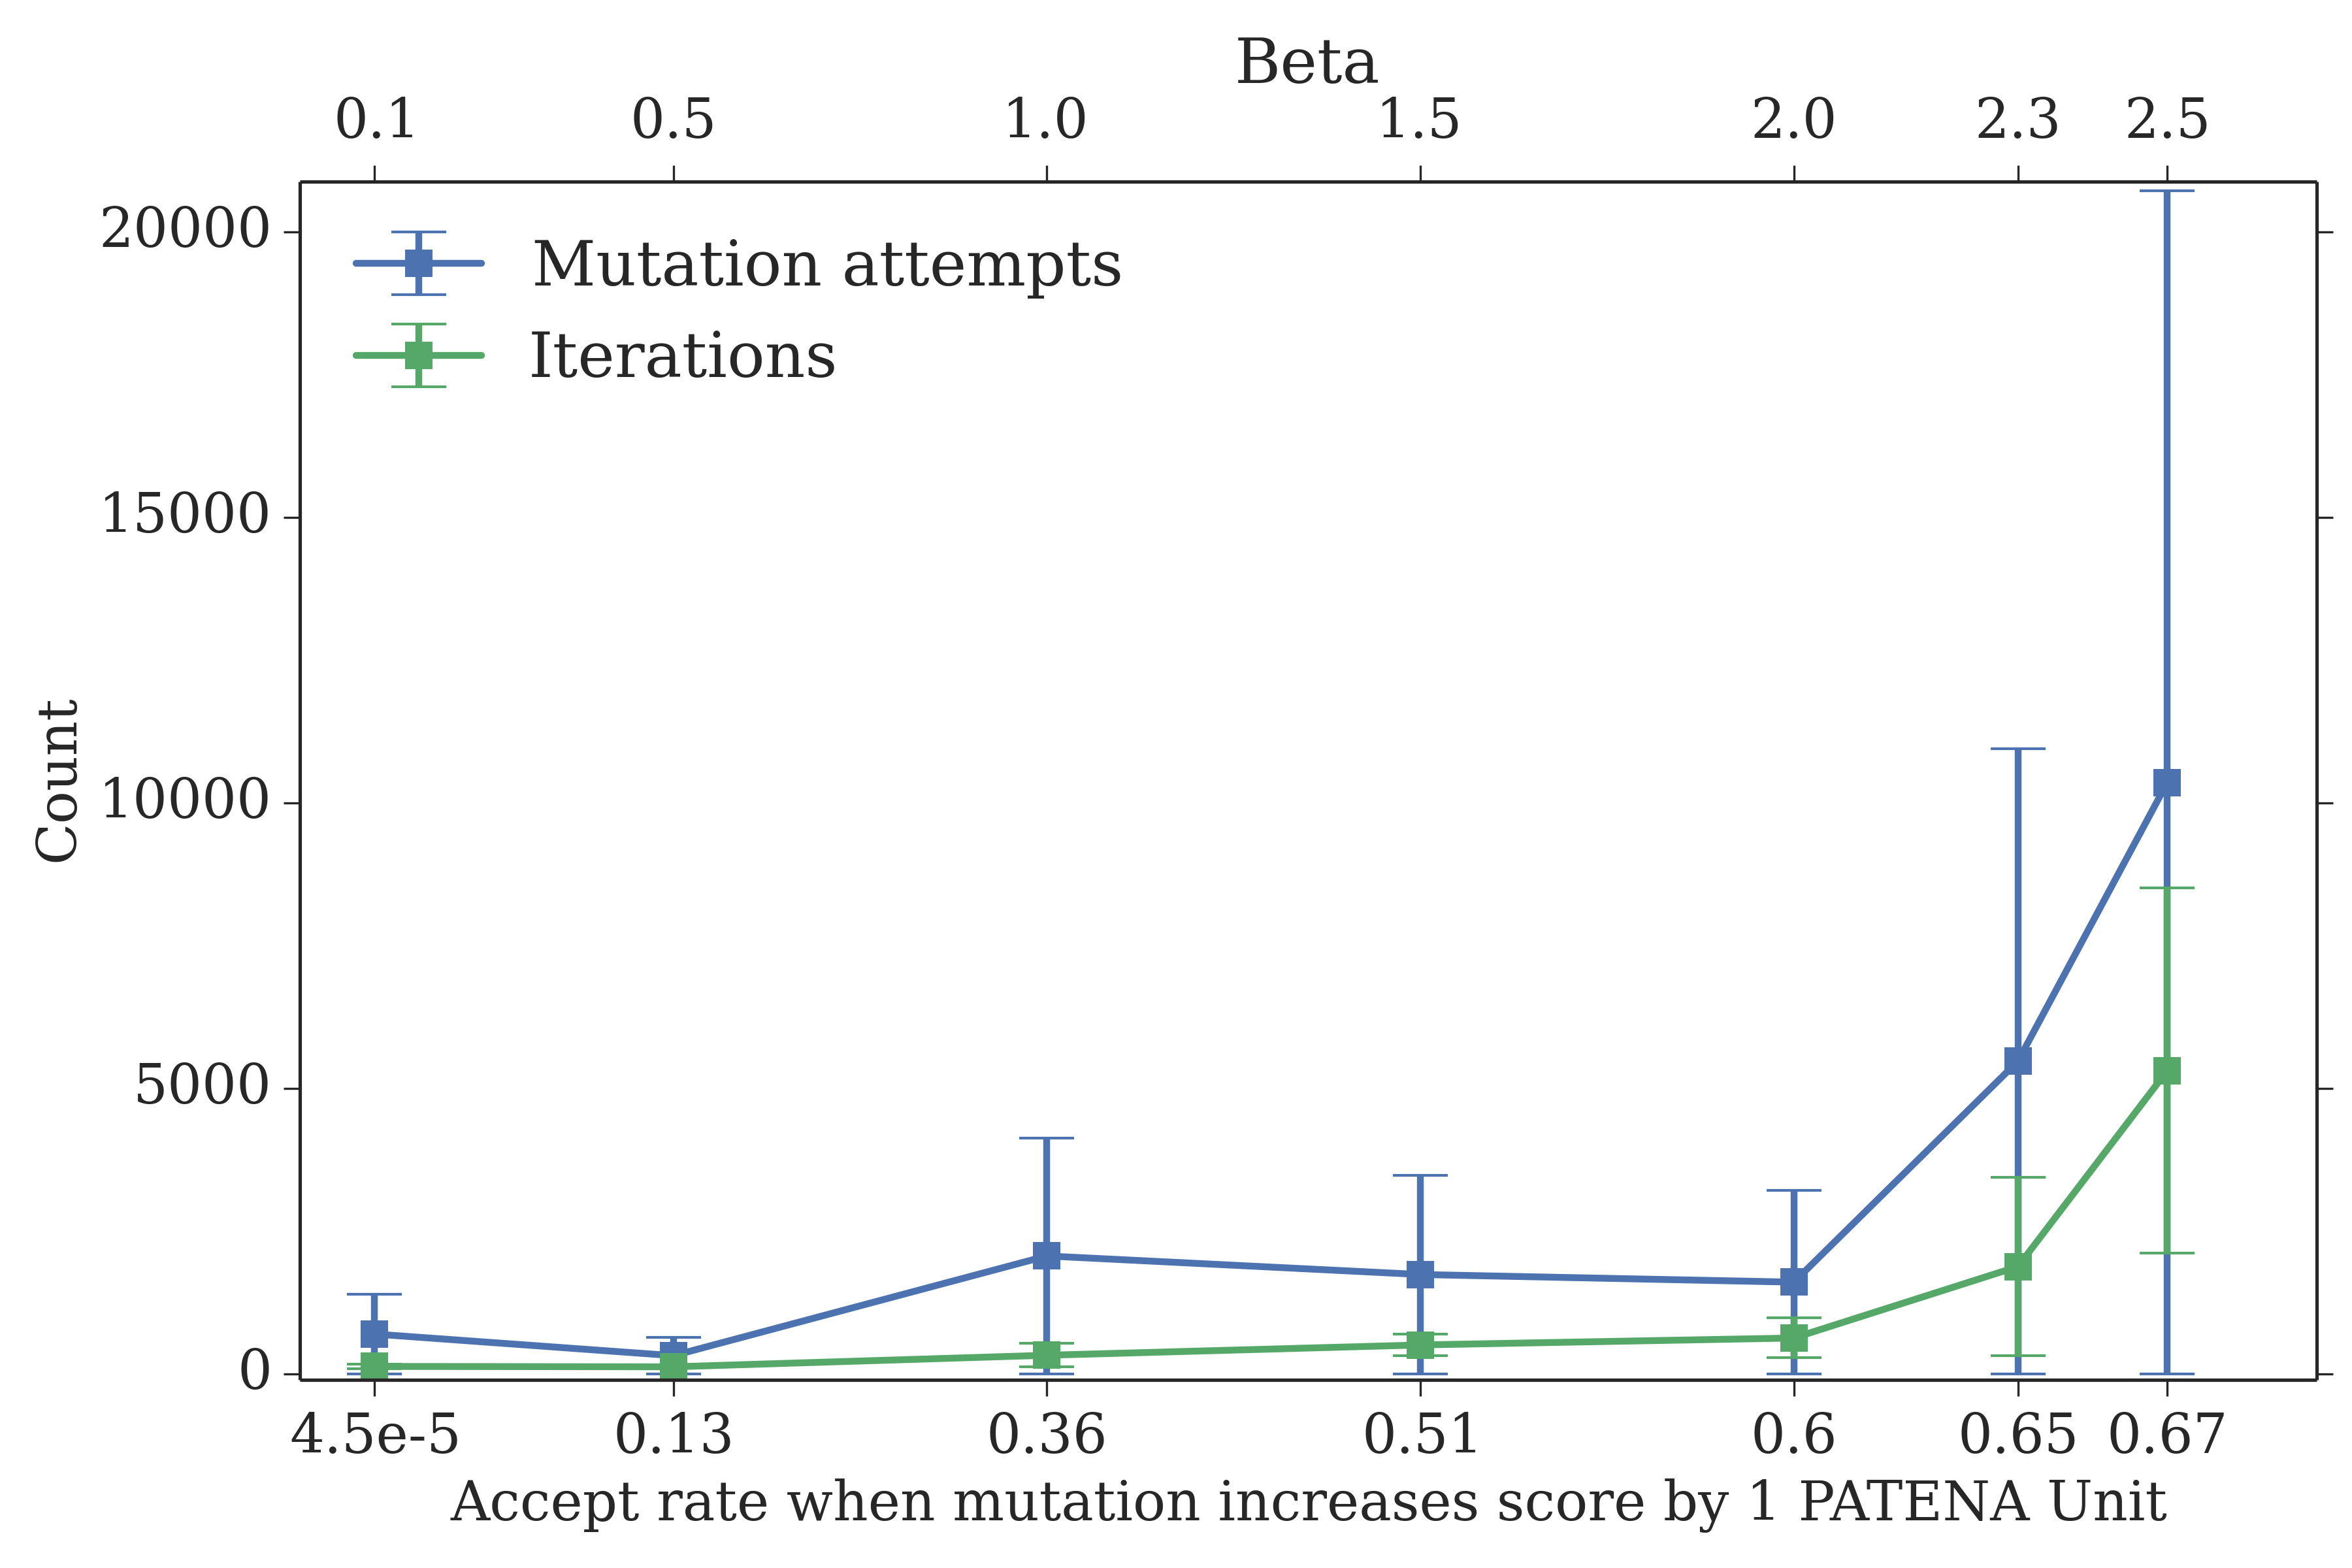
\includegraphics[width=340px,height=250px]{../img/beta-vs-Mut-iterations}\\
\end{adjustwidth}
\end{frame}











% *************************************************************
%     ITERATION vs MUT. ATTEMPTS(MEAN)
% *************************************************************
\begin{frame}
\begin{adjustwidth}{-2.0em}{-2.0em}
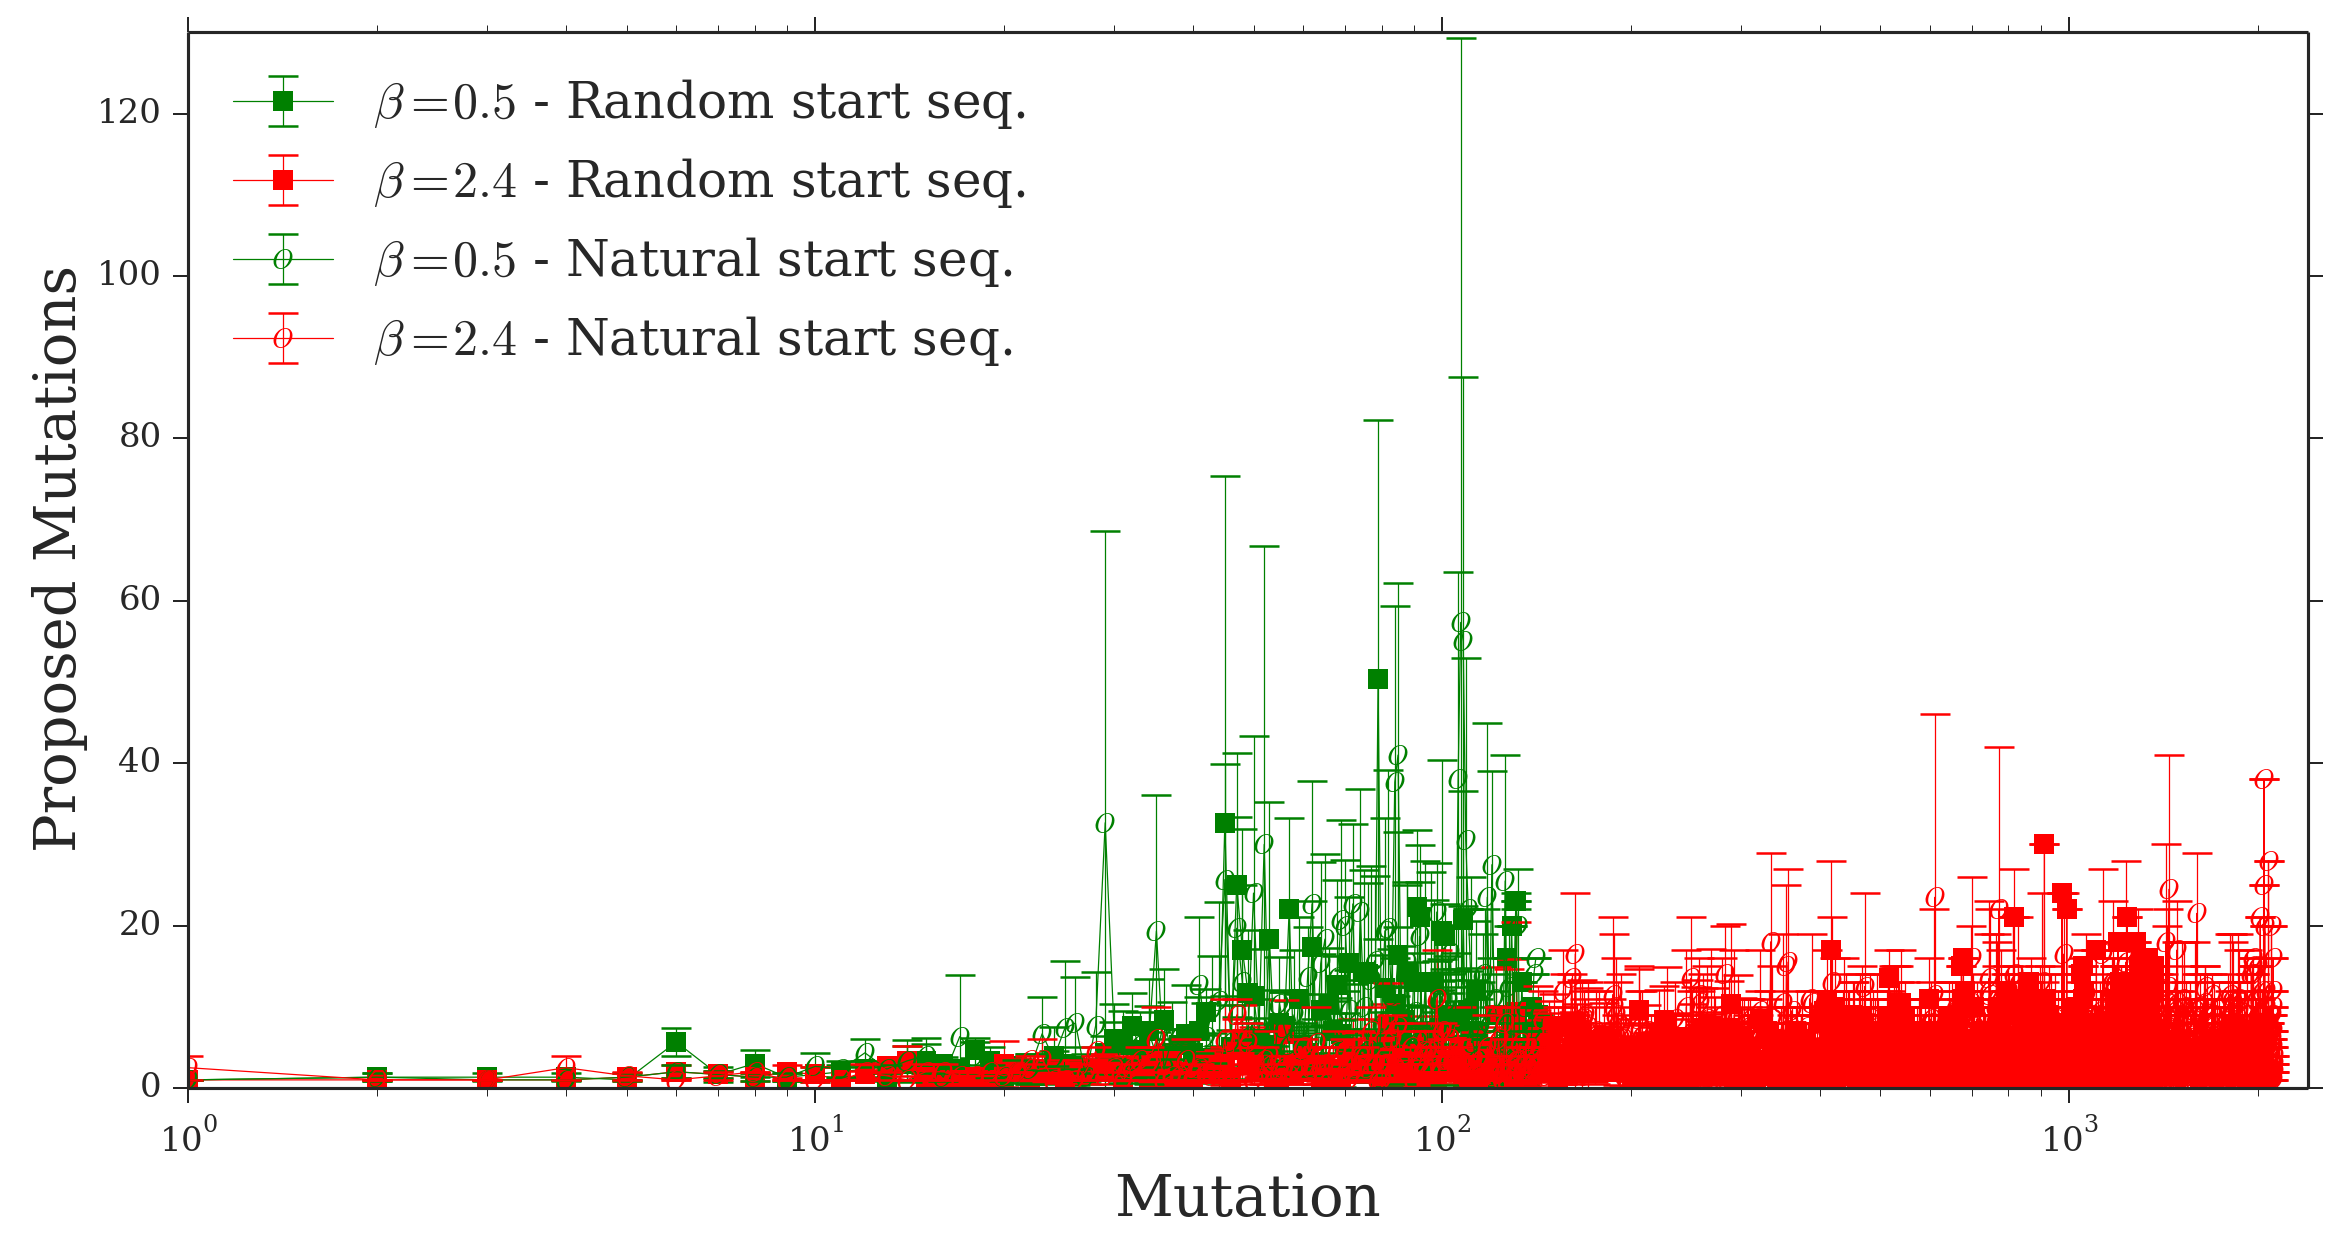
\includegraphics[width=340px,height=250px]{../img/iterationVsMutAttempts-mean.png} 
\end{adjustwidth}
\end{frame}









% 
% \begin{frame}
% \centering
% Fixed starting sequence $\rightarrow$ 74 designs \\
% \begin{adjustwidth}{-1.5em}{-2.5em}
% 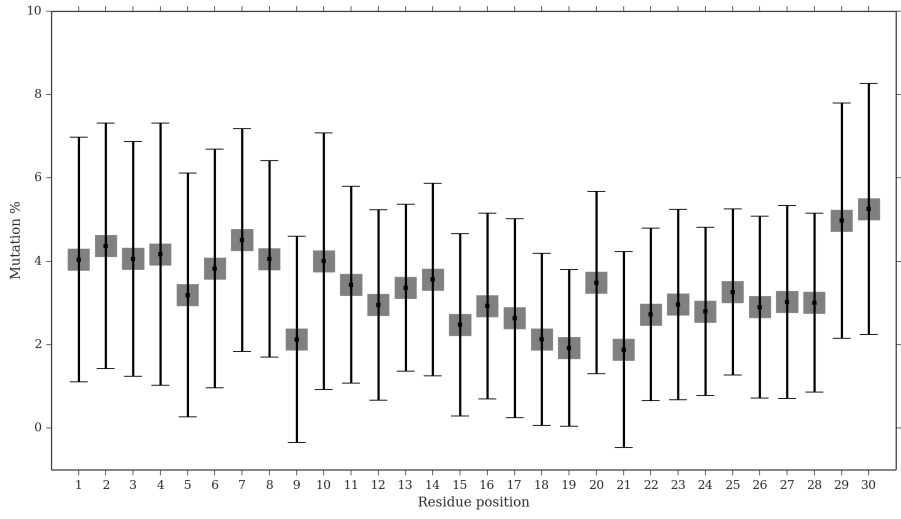
\includegraphics[width=340px,height=150px]{../img/mutationsPerPosition.png}\\ 
% % \vspace{10px}
% \hspace{25px}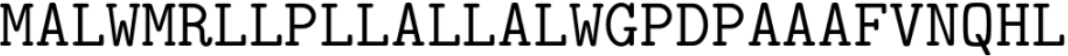
\includegraphics[width=310px,height=10px]{../img/sequence.png}
% \end{adjustwidth}
% \end{frame}
% 





\begin{frame}
\centering
Fixed starting sequence $\rightarrow$ 74 designs - Beta 0.5 , 0.1\\

\begin{adjustwidth}{-1.5em}{-2.5em}
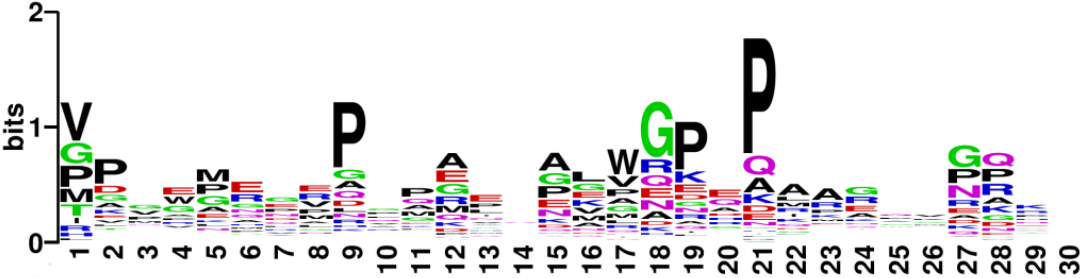
\includegraphics[width=340px,height=80px]{../img/logo.png}\\ 
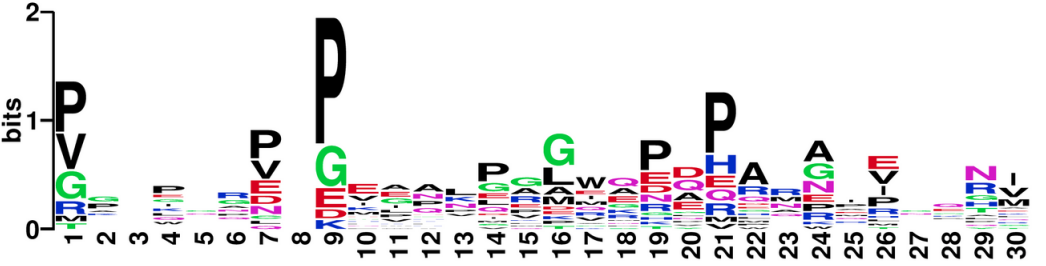
\includegraphics[width=345px,height=80px]{../img/logoBeta0-1.png}\\ 
\vspace{5px}
\hspace{18px}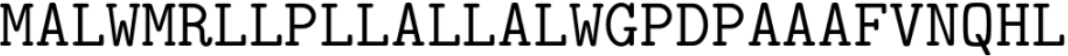
\includegraphics[width=324px,height=15px]{../img/sequence.png}
\end{adjustwidth}
\end{frame}











% The name
\begin{frame}{Limpio como una patena}
\centering
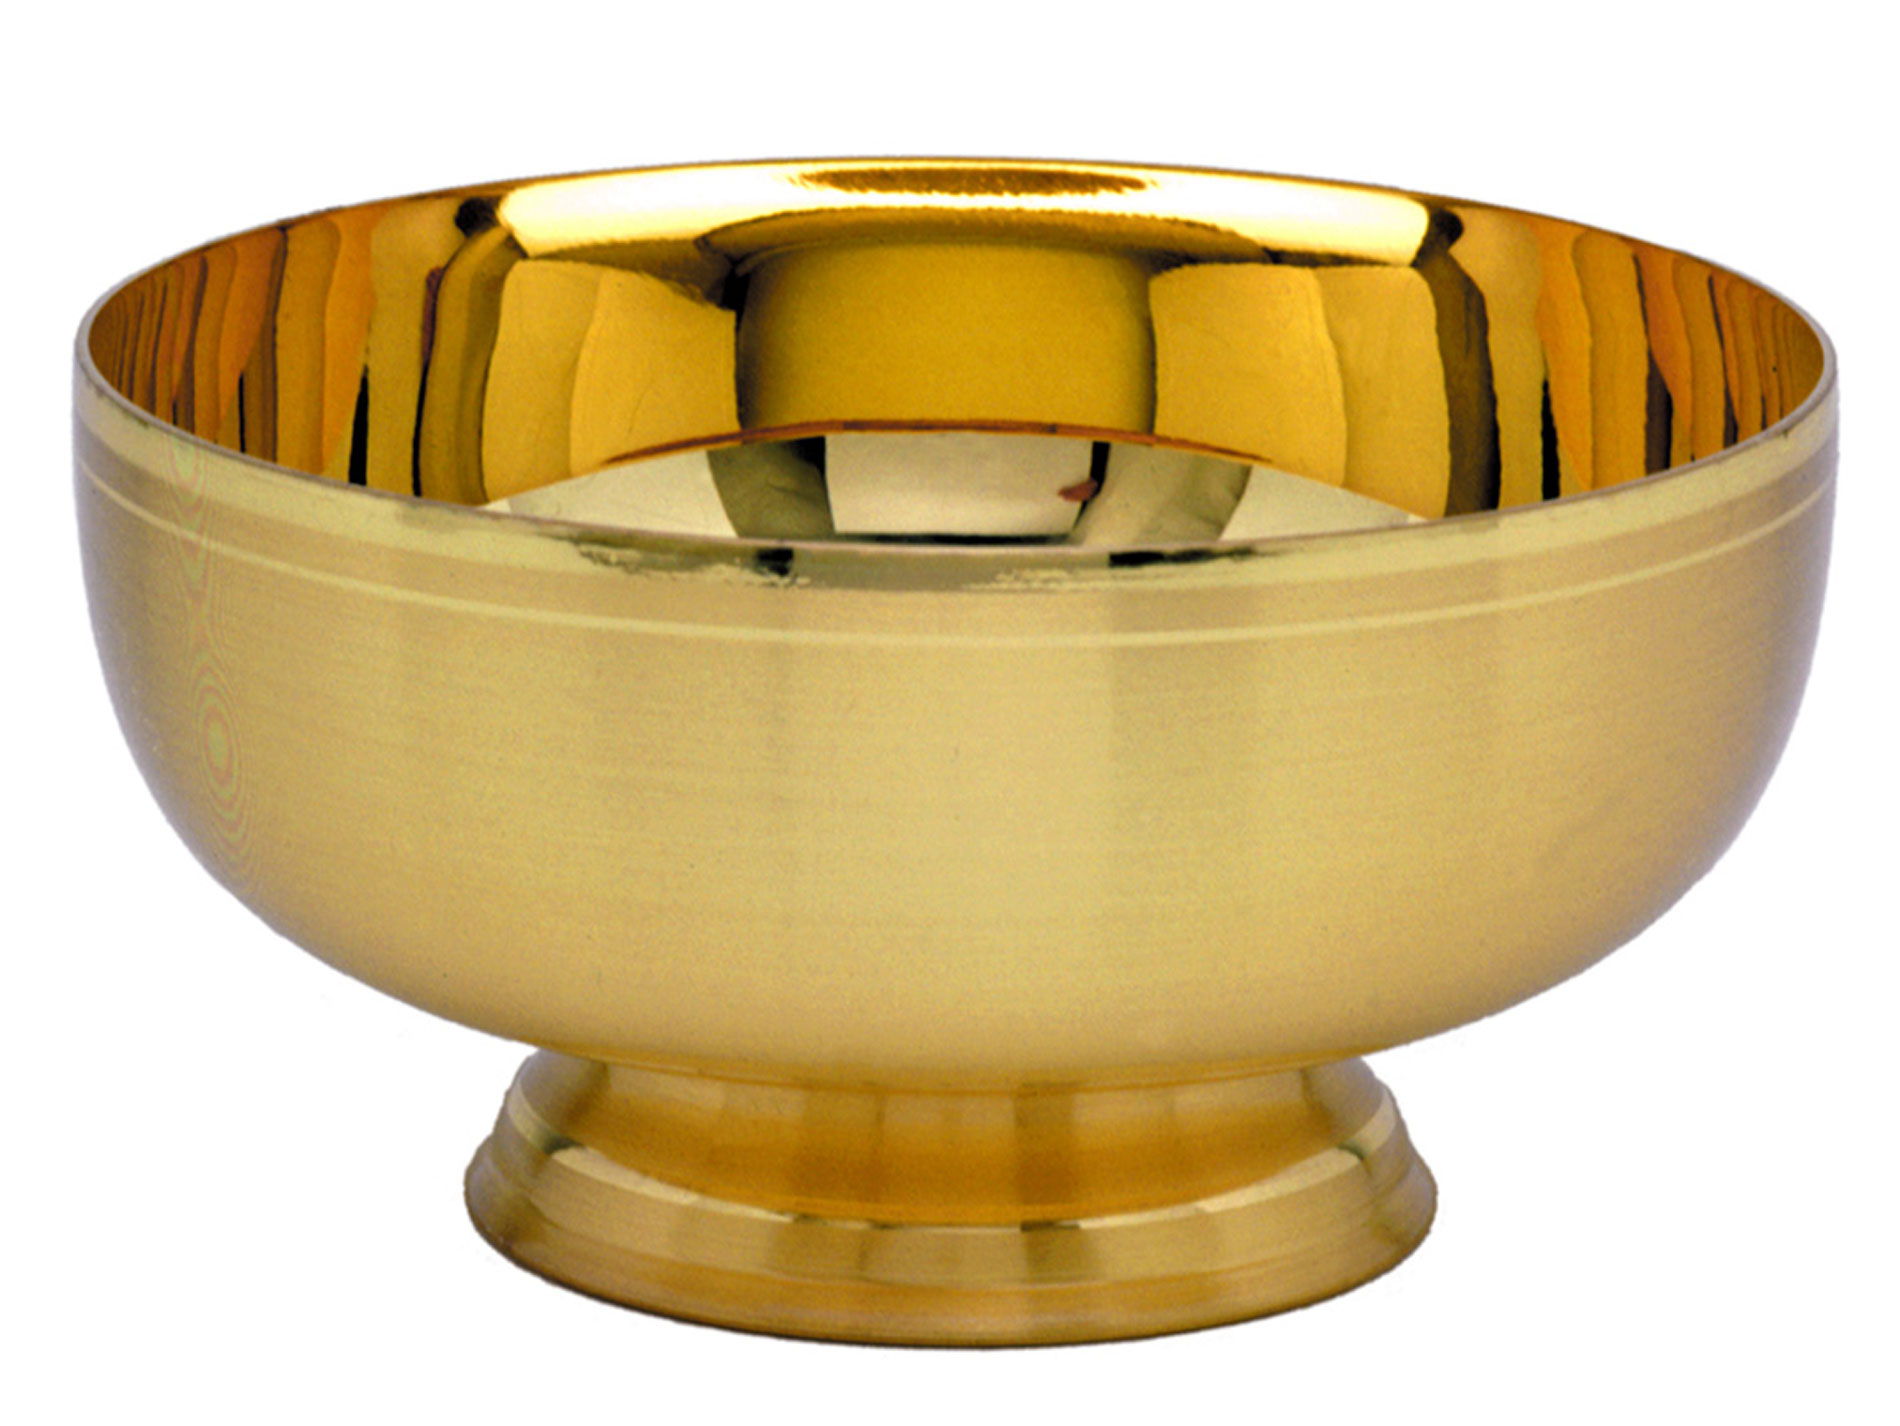
\includegraphics[width=300px]{../img/patena.jpg}
\end{frame}


\end{document}

